\documentclass[twoside]{book}

% Packages required by doxygen
\usepackage{calc}
\usepackage{doxygen}
\usepackage{graphicx}
\usepackage[utf8]{inputenc}
\usepackage{makeidx}
\usepackage{multicol}
\usepackage{multirow}
\usepackage{textcomp}
\usepackage[table]{xcolor}

% Font selection
\usepackage[T1]{fontenc}
\usepackage{mathptmx}
\usepackage[scaled=.90]{helvet}
\usepackage{courier}
\usepackage{amssymb}
\usepackage{sectsty}
\renewcommand{\familydefault}{\sfdefault}
\allsectionsfont{%
  \fontseries{bc}\selectfont%
  \color{darkgray}%
}
\renewcommand{\DoxyLabelFont}{%
  \fontseries{bc}\selectfont%
  \color{darkgray}%
}

% Page & text layout
\usepackage{geometry}
\geometry{%
  a4paper,%
  top=2.5cm,%
  bottom=2.5cm,%
  left=2.5cm,%
  right=2.5cm%
}
\tolerance=750
\hfuzz=15pt
\hbadness=750
\setlength{\emergencystretch}{15pt}
\setlength{\parindent}{0cm}
\setlength{\parskip}{0.2cm}
\makeatletter
\renewcommand{\paragraph}{%
  \@startsection{paragraph}{4}{0ex}{-1.0ex}{1.0ex}{%
    \normalfont\normalsize\bfseries\SS@parafont%
  }%
}
\renewcommand{\subparagraph}{%
  \@startsection{subparagraph}{5}{0ex}{-1.0ex}{1.0ex}{%
    \normalfont\normalsize\bfseries\SS@subparafont%
  }%
}
\makeatother

% Headers & footers
\usepackage{fancyhdr}
\pagestyle{fancyplain}
\fancyhead[LE]{\fancyplain{}{\bfseries\thepage}}
\fancyhead[CE]{\fancyplain{}{}}
\fancyhead[RE]{\fancyplain{}{\bfseries\leftmark}}
\fancyhead[LO]{\fancyplain{}{\bfseries\rightmark}}
\fancyhead[CO]{\fancyplain{}{}}
\fancyhead[RO]{\fancyplain{}{\bfseries\thepage}}
\fancyfoot[LE]{\fancyplain{}{}}
\fancyfoot[CE]{\fancyplain{}{}}
\fancyfoot[RE]{\fancyplain{}{\bfseries\scriptsize Generated on Tue Oct 30 2018 22\-:54\-:42 for editor by Doxygen }}
\fancyfoot[LO]{\fancyplain{}{\bfseries\scriptsize Generated on Tue Oct 30 2018 22\-:54\-:42 for editor by Doxygen }}
\fancyfoot[CO]{\fancyplain{}{}}
\fancyfoot[RO]{\fancyplain{}{}}
\renewcommand{\footrulewidth}{0.4pt}
\renewcommand{\chaptermark}[1]{%
  \markboth{#1}{}%
}
\renewcommand{\sectionmark}[1]{%
  \markright{\thesection\ #1}%
}

% Indices & bibliography
\usepackage{natbib}
\usepackage[titles]{tocloft}
\setcounter{tocdepth}{3}
\setcounter{secnumdepth}{5}
\makeindex

% Hyperlinks (required, but should be loaded last)
\usepackage{ifpdf}
\ifpdf
  \usepackage[pdftex,pagebackref=true]{hyperref}
\else
  \usepackage[ps2pdf,pagebackref=true]{hyperref}
\fi
\hypersetup{%
  colorlinks=true,%
  linkcolor=blue,%
  citecolor=blue,%
  unicode%
}

% Custom commands
\newcommand{\clearemptydoublepage}{%
  \newpage{\pagestyle{empty}\cleardoublepage}%
}


%===== C O N T E N T S =====

\begin{document}

% Titlepage & ToC
\hypersetup{pageanchor=false}
\pagenumbering{roman}
\begin{titlepage}
\vspace*{7cm}
\begin{center}%
{\Large editor }\\
\vspace*{1cm}
{\large Generated by Doxygen 1.8.6}\\
\vspace*{0.5cm}
{\small Tue Oct 30 2018 22:54:42}\\
\end{center}
\end{titlepage}
\clearemptydoublepage
\tableofcontents
\clearemptydoublepage
\pagenumbering{arabic}
\hypersetup{pageanchor=true}

%--- Begin generated contents ---
\chapter{Условие}
\label{md__r_e_a_d_m_e}
\hypertarget{md__r_e_a_d_m_e}{}
Спроектировать простейший графический векторный редактор. Подготовить макеты классов отражающих структуру будущего проекта.

Функционал для макетирования следующй\-:
\begin{DoxyItemize}
\item создание нового документа
\item импорт документа из файла
\item экспорт документа в файл
\item создание графического примитива
\item удаление графического примитива
\end{DoxyItemize}

Основной упор сделать на шаблон контроллера и полиморфизм. Функции являющиеся обработчками G\-U\-I собрать в одном файле с функцией main.

\section*{Требования к реализации}

Внимание должен быть сосредоточено на декларациях, реализация только в крайнем случае для минимальной демонстрации необходимых вызовов.

Проект должен компилироваться, все заголовки должны пройти стадию компиляции.

Результатом работы должен быть каталог с диаграммами опубликованный на github-\/pages.

\section*{Проверка}

Задание считается выполненным успешно, если все файлы прошли стадию компиляции, все классы охвачены диаграммами, код успешно прошел анализ. 
\chapter{Hierarchical Index}
\section{Class Hierarchy}
This inheritance list is sorted roughly, but not completely, alphabetically\-:\begin{DoxyCompactList}
\item \contentsline{section}{editor}{\pageref{structeditor}}{}
\item \contentsline{section}{Enum\-Class\-Hash}{\pageref{struct_enum_class_hash}}{}
\item \contentsline{section}{I\-Observer}{\pageref{class_i_observer}}{}
\begin{DoxyCompactList}
\item \contentsline{section}{View}{\pageref{class_view}}{}
\end{DoxyCompactList}
\item \contentsline{section}{Observable}{\pageref{class_observable}}{}
\begin{DoxyCompactList}
\item \contentsline{section}{Model}{\pageref{class_model}}{}
\end{DoxyCompactList}
\item \contentsline{section}{Shape}{\pageref{class_shape}}{}
\begin{DoxyCompactList}
\item \contentsline{section}{Circle}{\pageref{class_circle}}{}
\item \contentsline{section}{Ellipse}{\pageref{class_ellipse}}{}
\item \contentsline{section}{Square}{\pageref{class_square}}{}
\end{DoxyCompactList}
\item \contentsline{section}{Shape\-Factory}{\pageref{class_shape_factory}}{}
\item \contentsline{section}{Shape\-Factory\-Register}{\pageref{struct_shape_factory_register}}{}
\end{DoxyCompactList}

\chapter{Class Index}
\section{Class List}
Here are the classes, structs, unions and interfaces with brief descriptions\-:\begin{DoxyCompactList}
\item\contentsline{section}{\hyperlink{class_circle}{Circle} }{\pageref{class_circle}}{}
\item\contentsline{section}{\hyperlink{class_controller}{Controller} }{\pageref{class_controller}}{}
\item\contentsline{section}{\hyperlink{structeditor}{editor} }{\pageref{structeditor}}{}
\item\contentsline{section}{\hyperlink{class_ellipse}{Ellipse} }{\pageref{class_ellipse}}{}
\item\contentsline{section}{\hyperlink{struct_enum_class_hash}{Enum\-Class\-Hash} }{\pageref{struct_enum_class_hash}}{}
\item\contentsline{section}{\hyperlink{class_i_observer}{I\-Observer} }{\pageref{class_i_observer}}{}
\item\contentsline{section}{\hyperlink{class_model}{Model} }{\pageref{class_model}}{}
\item\contentsline{section}{\hyperlink{class_observable}{Observable} }{\pageref{class_observable}}{}
\item\contentsline{section}{\hyperlink{class_shape}{Shape} }{\pageref{class_shape}}{}
\item\contentsline{section}{\hyperlink{class_shape_factory}{Shape\-Factory} }{\pageref{class_shape_factory}}{}
\item\contentsline{section}{\hyperlink{struct_shape_factory_register}{Shape\-Factory\-Register} }{\pageref{struct_shape_factory_register}}{}
\item\contentsline{section}{\hyperlink{class_square}{Square} }{\pageref{class_square}}{}
\item\contentsline{section}{\hyperlink{class_view}{View} }{\pageref{class_view}}{}
\end{DoxyCompactList}

\chapter{File Index}
\section{File List}
Here is a list of all files with brief descriptions\-:\begin{DoxyCompactList}
\item\contentsline{section}{C\-Make\-Files/\hyperlink{feature__tests_8c}{feature\-\_\-tests.\-c} }{\pageref{feature__tests_8c}}{}
\item\contentsline{section}{C\-Make\-Files/\hyperlink{feature__tests_8cxx}{feature\-\_\-tests.\-cxx} }{\pageref{feature__tests_8cxx}}{}
\item\contentsline{section}{C\-Make\-Files/3.\-9.\-2/\-Compiler\-Id\-C/\hyperlink{_c_make_c_compiler_id_8c}{C\-Make\-C\-Compiler\-Id.\-c} }{\pageref{_c_make_c_compiler_id_8c}}{}
\item\contentsline{section}{C\-Make\-Files/3.\-9.\-2/\-Compiler\-Id\-C\-X\-X/\hyperlink{_c_make_c_x_x_compiler_id_8cpp}{C\-Make\-C\-X\-X\-Compiler\-Id.\-cpp} }{\pageref{_c_make_c_x_x_compiler_id_8cpp}}{}
\item\contentsline{section}{src/\hyperlink{main_8cpp}{main.\-cpp} }{\pageref{main_8cpp}}{}
\item\contentsline{section}{src/include/\hyperlink{controller_8h}{controller.\-h} }{\pageref{controller_8h}}{}
\item\contentsline{section}{src/include/\hyperlink{model_8h}{model.\-h} }{\pageref{model_8h}}{}
\item\contentsline{section}{src/include/\hyperlink{observer_8h}{observer.\-h} }{\pageref{observer_8h}}{}
\item\contentsline{section}{src/include/\hyperlink{shape_8h}{shape.\-h} }{\pageref{shape_8h}}{}
\item\contentsline{section}{src/include/\hyperlink{stdafx_8h}{stdafx.\-h} }{\pageref{stdafx_8h}}{}
\item\contentsline{section}{src/include/\hyperlink{view_8h}{view.\-h} }{\pageref{view_8h}}{}
\item\contentsline{section}{test/\hyperlink{test__shape__factory_8cpp}{test\-\_\-shape\-\_\-factory.\-cpp} }{\pageref{test__shape__factory_8cpp}}{}
\end{DoxyCompactList}

\chapter{Class Documentation}
\hypertarget{class_circle}{\section{Circle Class Reference}
\label{class_circle}\index{Circle@{Circle}}
}


{\ttfamily \#include $<$shape.\-h$>$}



Inheritance diagram for Circle\-:
\nopagebreak
\begin{figure}[H]
\begin{center}
\leavevmode
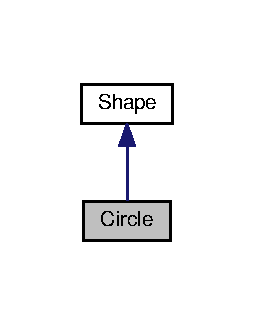
\includegraphics[width=122pt]{class_circle__inherit__graph}
\end{center}
\end{figure}


Collaboration diagram for Circle\-:
\nopagebreak
\begin{figure}[H]
\begin{center}
\leavevmode
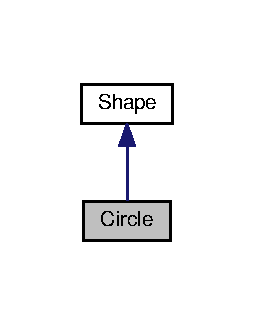
\includegraphics[width=122pt]{class_circle__coll__graph}
\end{center}
\end{figure}
\subsection*{Public Member Functions}
\begin{DoxyCompactItemize}
\item 
\hyperlink{class_circle_aacd40dfd23f14473402390dada4d5083}{Circle} (uint32\-\_\-t x, uint32\-\_\-t y, uint32\-\_\-t r)
\item 
void \hyperlink{class_circle_a3a3f7166e7f629e44f9044b0e537eb22}{draw} ()
\end{DoxyCompactItemize}
\subsection*{Static Public Member Functions}
\begin{DoxyCompactItemize}
\item 
static std\-::shared\-\_\-ptr$<$ \hyperlink{class_shape}{Shape} $>$ \hyperlink{class_circle_a24650041916815e42f19b0ba0820cc3c}{create} (uint32\-\_\-t x, uint32\-\_\-t y, uint32\-\_\-t r)
\end{DoxyCompactItemize}
\subsection*{Additional Inherited Members}


\subsection{Constructor \& Destructor Documentation}
\hypertarget{class_circle_aacd40dfd23f14473402390dada4d5083}{\index{Circle@{Circle}!Circle@{Circle}}
\index{Circle@{Circle}!Circle@{Circle}}
\subsubsection[{Circle}]{\setlength{\rightskip}{0pt plus 5cm}Circle\-::\-Circle (
\begin{DoxyParamCaption}
\item[{uint32\-\_\-t}]{x, }
\item[{uint32\-\_\-t}]{y, }
\item[{uint32\-\_\-t}]{r}
\end{DoxyParamCaption}
)\hspace{0.3cm}{\ttfamily [inline]}}}\label{class_circle_aacd40dfd23f14473402390dada4d5083}


\subsection{Member Function Documentation}
\hypertarget{class_circle_a24650041916815e42f19b0ba0820cc3c}{\index{Circle@{Circle}!create@{create}}
\index{create@{create}!Circle@{Circle}}
\subsubsection[{create}]{\setlength{\rightskip}{0pt plus 5cm}static std\-::shared\-\_\-ptr$<${\bf Shape}$>$ Circle\-::create (
\begin{DoxyParamCaption}
\item[{uint32\-\_\-t}]{x, }
\item[{uint32\-\_\-t}]{y, }
\item[{uint32\-\_\-t}]{r}
\end{DoxyParamCaption}
)\hspace{0.3cm}{\ttfamily [inline]}, {\ttfamily [static]}}}\label{class_circle_a24650041916815e42f19b0ba0820cc3c}
\hypertarget{class_circle_a3a3f7166e7f629e44f9044b0e537eb22}{\index{Circle@{Circle}!draw@{draw}}
\index{draw@{draw}!Circle@{Circle}}
\subsubsection[{draw}]{\setlength{\rightskip}{0pt plus 5cm}void Circle\-::draw (
\begin{DoxyParamCaption}
{}
\end{DoxyParamCaption}
)\hspace{0.3cm}{\ttfamily [inline]}, {\ttfamily [virtual]}}}\label{class_circle_a3a3f7166e7f629e44f9044b0e537eb22}


Implements \hyperlink{class_shape_afacc5aad8e37308c3ce8fef768199b05}{Shape}.



The documentation for this class was generated from the following file\-:\begin{DoxyCompactItemize}
\item 
src/include/\hyperlink{shape_8h}{shape.\-h}\end{DoxyCompactItemize}

\hypertarget{class_controller}{\section{Controller Class Reference}
\label{class_controller}\index{Controller@{Controller}}
}


{\ttfamily \#include $<$controller.\-h$>$}

\subsection*{Public Member Functions}
\begin{DoxyCompactItemize}
\item 
\hyperlink{class_controller_a09ed75adac2db59f6a55130b734a5798}{Controller} (std\-::shared\-\_\-ptr$<$ \hyperlink{class_view}{View} $>$ view, std\-::shared\-\_\-ptr$<$ \hyperlink{class_model}{Model} $>$ model)
\item 
void \hyperlink{class_controller_a6fe322152f86d083d22473753fb357fb}{save\-As} (std\-::string file\-\_\-name)
\item 
void \hyperlink{class_controller_ae0f9dec048daf5dfdd42b82072ac6185}{save} ()
\item 
void \hyperlink{class_controller_a4168a80c0b5346408156997e1f89d75b}{close} ()
\item 
void \hyperlink{class_controller_a455fe9fe6d025f957df000f9636bc9a5}{load\-File} (std\-::string file\-\_\-name)
\item 
void \hyperlink{class_controller_a361ed5314423517d3d5c1fb7e92f1623}{add\-Shape} (std\-::shared\-\_\-ptr$<$ \hyperlink{class_shape}{Shape} $>$ s)
\item 
void \hyperlink{class_controller_a31d66b8d2e987c91011c8a86acea7378}{remove\-Shape} (uint32\-\_\-t id)
\end{DoxyCompactItemize}


\subsection{Constructor \& Destructor Documentation}
\hypertarget{class_controller_a09ed75adac2db59f6a55130b734a5798}{\index{Controller@{Controller}!Controller@{Controller}}
\index{Controller@{Controller}!Controller@{Controller}}
\subsubsection[{Controller}]{\setlength{\rightskip}{0pt plus 5cm}Controller\-::\-Controller (
\begin{DoxyParamCaption}
\item[{std\-::shared\-\_\-ptr$<$ {\bf View} $>$}]{view, }
\item[{std\-::shared\-\_\-ptr$<$ {\bf Model} $>$}]{model}
\end{DoxyParamCaption}
)\hspace{0.3cm}{\ttfamily [inline]}}}\label{class_controller_a09ed75adac2db59f6a55130b734a5798}


\subsection{Member Function Documentation}
\hypertarget{class_controller_a361ed5314423517d3d5c1fb7e92f1623}{\index{Controller@{Controller}!add\-Shape@{add\-Shape}}
\index{add\-Shape@{add\-Shape}!Controller@{Controller}}
\subsubsection[{add\-Shape}]{\setlength{\rightskip}{0pt plus 5cm}void Controller\-::add\-Shape (
\begin{DoxyParamCaption}
\item[{std\-::shared\-\_\-ptr$<$ {\bf Shape} $>$}]{s}
\end{DoxyParamCaption}
)\hspace{0.3cm}{\ttfamily [inline]}}}\label{class_controller_a361ed5314423517d3d5c1fb7e92f1623}
\hypertarget{class_controller_a4168a80c0b5346408156997e1f89d75b}{\index{Controller@{Controller}!close@{close}}
\index{close@{close}!Controller@{Controller}}
\subsubsection[{close}]{\setlength{\rightskip}{0pt plus 5cm}void Controller\-::close (
\begin{DoxyParamCaption}
{}
\end{DoxyParamCaption}
)\hspace{0.3cm}{\ttfamily [inline]}}}\label{class_controller_a4168a80c0b5346408156997e1f89d75b}
\hypertarget{class_controller_a455fe9fe6d025f957df000f9636bc9a5}{\index{Controller@{Controller}!load\-File@{load\-File}}
\index{load\-File@{load\-File}!Controller@{Controller}}
\subsubsection[{load\-File}]{\setlength{\rightskip}{0pt plus 5cm}void Controller\-::load\-File (
\begin{DoxyParamCaption}
\item[{std\-::string}]{file\-\_\-name}
\end{DoxyParamCaption}
)\hspace{0.3cm}{\ttfamily [inline]}}}\label{class_controller_a455fe9fe6d025f957df000f9636bc9a5}
\hypertarget{class_controller_a31d66b8d2e987c91011c8a86acea7378}{\index{Controller@{Controller}!remove\-Shape@{remove\-Shape}}
\index{remove\-Shape@{remove\-Shape}!Controller@{Controller}}
\subsubsection[{remove\-Shape}]{\setlength{\rightskip}{0pt plus 5cm}void Controller\-::remove\-Shape (
\begin{DoxyParamCaption}
\item[{uint32\-\_\-t}]{id}
\end{DoxyParamCaption}
)\hspace{0.3cm}{\ttfamily [inline]}}}\label{class_controller_a31d66b8d2e987c91011c8a86acea7378}
\hypertarget{class_controller_ae0f9dec048daf5dfdd42b82072ac6185}{\index{Controller@{Controller}!save@{save}}
\index{save@{save}!Controller@{Controller}}
\subsubsection[{save}]{\setlength{\rightskip}{0pt plus 5cm}void Controller\-::save (
\begin{DoxyParamCaption}
{}
\end{DoxyParamCaption}
)\hspace{0.3cm}{\ttfamily [inline]}}}\label{class_controller_ae0f9dec048daf5dfdd42b82072ac6185}
\hypertarget{class_controller_a6fe322152f86d083d22473753fb357fb}{\index{Controller@{Controller}!save\-As@{save\-As}}
\index{save\-As@{save\-As}!Controller@{Controller}}
\subsubsection[{save\-As}]{\setlength{\rightskip}{0pt plus 5cm}void Controller\-::save\-As (
\begin{DoxyParamCaption}
\item[{std\-::string}]{file\-\_\-name}
\end{DoxyParamCaption}
)\hspace{0.3cm}{\ttfamily [inline]}}}\label{class_controller_a6fe322152f86d083d22473753fb357fb}


The documentation for this class was generated from the following file\-:\begin{DoxyCompactItemize}
\item 
src/include/\hyperlink{controller_8h}{controller.\-h}\end{DoxyCompactItemize}

\hypertarget{structeditor}{\section{editor Struct Reference}
\label{structeditor}\index{editor@{editor}}
}


The documentation for this struct was generated from the following file\-:\begin{DoxyCompactItemize}
\item 
src/\hyperlink{main_8cpp}{main.\-cpp}\end{DoxyCompactItemize}

\hypertarget{class_ellipse}{\section{Ellipse Class Reference}
\label{class_ellipse}\index{Ellipse@{Ellipse}}
}


{\ttfamily \#include $<$shape.\-h$>$}



Inheritance diagram for Ellipse\-:
\nopagebreak
\begin{figure}[H]
\begin{center}
\leavevmode
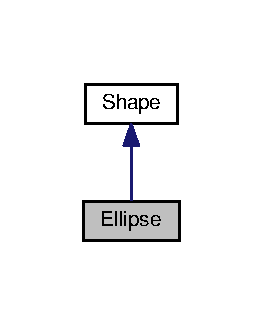
\includegraphics[width=126pt]{class_ellipse__inherit__graph}
\end{center}
\end{figure}


Collaboration diagram for Ellipse\-:
\nopagebreak
\begin{figure}[H]
\begin{center}
\leavevmode
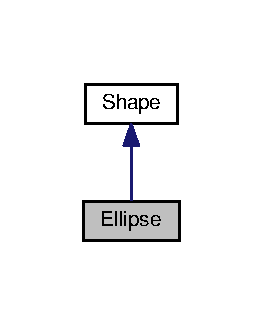
\includegraphics[width=126pt]{class_ellipse__coll__graph}
\end{center}
\end{figure}
\subsection*{Public Member Functions}
\begin{DoxyCompactItemize}
\item 
\hyperlink{class_ellipse_a207fe9e5c684498eb017ae3b5034e4dd}{Ellipse} (uint32\-\_\-t x1, uint32\-\_\-t y1, uint32\-\_\-t x2, uint32\-\_\-t y2, uint32\-\_\-t r)
\item 
void \hyperlink{class_ellipse_a312c0cf0e855dc79d37c07ec52bf202e}{draw} ()
\end{DoxyCompactItemize}
\subsection*{Static Public Member Functions}
\begin{DoxyCompactItemize}
\item 
static std\-::shared\-\_\-ptr$<$ \hyperlink{class_shape}{Shape} $>$ \hyperlink{class_ellipse_a2984a70d775908fe1dabdcb51c7054c4}{create} (uint32\-\_\-t x1, uint32\-\_\-t y1, uint32\-\_\-t x2, uint32\-\_\-t y2, uint32\-\_\-t r)
\end{DoxyCompactItemize}
\subsection*{Additional Inherited Members}


\subsection{Constructor \& Destructor Documentation}
\hypertarget{class_ellipse_a207fe9e5c684498eb017ae3b5034e4dd}{\index{Ellipse@{Ellipse}!Ellipse@{Ellipse}}
\index{Ellipse@{Ellipse}!Ellipse@{Ellipse}}
\subsubsection[{Ellipse}]{\setlength{\rightskip}{0pt plus 5cm}Ellipse\-::\-Ellipse (
\begin{DoxyParamCaption}
\item[{uint32\-\_\-t}]{x1, }
\item[{uint32\-\_\-t}]{y1, }
\item[{uint32\-\_\-t}]{x2, }
\item[{uint32\-\_\-t}]{y2, }
\item[{uint32\-\_\-t}]{r}
\end{DoxyParamCaption}
)\hspace{0.3cm}{\ttfamily [inline]}}}\label{class_ellipse_a207fe9e5c684498eb017ae3b5034e4dd}


\subsection{Member Function Documentation}
\hypertarget{class_ellipse_a2984a70d775908fe1dabdcb51c7054c4}{\index{Ellipse@{Ellipse}!create@{create}}
\index{create@{create}!Ellipse@{Ellipse}}
\subsubsection[{create}]{\setlength{\rightskip}{0pt plus 5cm}static std\-::shared\-\_\-ptr$<${\bf Shape}$>$ Ellipse\-::create (
\begin{DoxyParamCaption}
\item[{uint32\-\_\-t}]{x1, }
\item[{uint32\-\_\-t}]{y1, }
\item[{uint32\-\_\-t}]{x2, }
\item[{uint32\-\_\-t}]{y2, }
\item[{uint32\-\_\-t}]{r}
\end{DoxyParamCaption}
)\hspace{0.3cm}{\ttfamily [inline]}, {\ttfamily [static]}}}\label{class_ellipse_a2984a70d775908fe1dabdcb51c7054c4}
\hypertarget{class_ellipse_a312c0cf0e855dc79d37c07ec52bf202e}{\index{Ellipse@{Ellipse}!draw@{draw}}
\index{draw@{draw}!Ellipse@{Ellipse}}
\subsubsection[{draw}]{\setlength{\rightskip}{0pt plus 5cm}void Ellipse\-::draw (
\begin{DoxyParamCaption}
{}
\end{DoxyParamCaption}
)\hspace{0.3cm}{\ttfamily [inline]}, {\ttfamily [virtual]}}}\label{class_ellipse_a312c0cf0e855dc79d37c07ec52bf202e}


Implements \hyperlink{class_shape_afacc5aad8e37308c3ce8fef768199b05}{Shape}.



The documentation for this class was generated from the following file\-:\begin{DoxyCompactItemize}
\item 
src/include/\hyperlink{shape_8h}{shape.\-h}\end{DoxyCompactItemize}

\hypertarget{struct_enum_class_hash}{\section{Enum\-Class\-Hash Struct Reference}
\label{struct_enum_class_hash}\index{Enum\-Class\-Hash@{Enum\-Class\-Hash}}
}


{\ttfamily \#include $<$shape.\-h$>$}

\subsection*{Public Member Functions}
\begin{DoxyCompactItemize}
\item 
{\footnotesize template$<$typename T $>$ }\\std\-::size\-\_\-t \hyperlink{struct_enum_class_hash_a02ef43aab3f3004ec306c58d3ebd423a}{operator()} (T t) const 
\end{DoxyCompactItemize}


\subsection{Member Function Documentation}
\hypertarget{struct_enum_class_hash_a02ef43aab3f3004ec306c58d3ebd423a}{\index{Enum\-Class\-Hash@{Enum\-Class\-Hash}!operator()@{operator()}}
\index{operator()@{operator()}!EnumClassHash@{Enum\-Class\-Hash}}
\subsubsection[{operator()}]{\setlength{\rightskip}{0pt plus 5cm}template$<$typename T $>$ std\-::size\-\_\-t Enum\-Class\-Hash\-::operator() (
\begin{DoxyParamCaption}
\item[{T}]{t}
\end{DoxyParamCaption}
) const\hspace{0.3cm}{\ttfamily [inline]}}}\label{struct_enum_class_hash_a02ef43aab3f3004ec306c58d3ebd423a}


The documentation for this struct was generated from the following file\-:\begin{DoxyCompactItemize}
\item 
src/include/\hyperlink{shape_8h}{shape.\-h}\end{DoxyCompactItemize}

\hypertarget{class_i_observer}{\section{I\-Observer Class Reference}
\label{class_i_observer}\index{I\-Observer@{I\-Observer}}
}


{\ttfamily \#include $<$observer.\-h$>$}



Inheritance diagram for I\-Observer\-:
\nopagebreak
\begin{figure}[H]
\begin{center}
\leavevmode
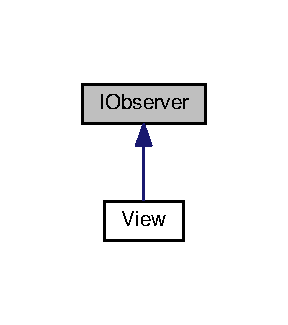
\includegraphics[width=138pt]{class_i_observer__inherit__graph}
\end{center}
\end{figure}
\subsection*{Public Member Functions}
\begin{DoxyCompactItemize}
\item 
virtual void \hyperlink{class_i_observer_a91a4770cbec97439f2faba69a1ed72e0}{update} ()=0
\item 
virtual \hyperlink{class_i_observer_a1306da2dbaf55620130af5586e3a0373}{$\sim$\-I\-Observer} ()=default
\end{DoxyCompactItemize}


\subsection{Constructor \& Destructor Documentation}
\hypertarget{class_i_observer_a1306da2dbaf55620130af5586e3a0373}{\index{I\-Observer@{I\-Observer}!$\sim$\-I\-Observer@{$\sim$\-I\-Observer}}
\index{$\sim$\-I\-Observer@{$\sim$\-I\-Observer}!IObserver@{I\-Observer}}
\subsubsection[{$\sim$\-I\-Observer}]{\setlength{\rightskip}{0pt plus 5cm}virtual I\-Observer\-::$\sim$\-I\-Observer (
\begin{DoxyParamCaption}
{}
\end{DoxyParamCaption}
)\hspace{0.3cm}{\ttfamily [virtual]}, {\ttfamily [default]}}}\label{class_i_observer_a1306da2dbaf55620130af5586e3a0373}


\subsection{Member Function Documentation}
\hypertarget{class_i_observer_a91a4770cbec97439f2faba69a1ed72e0}{\index{I\-Observer@{I\-Observer}!update@{update}}
\index{update@{update}!IObserver@{I\-Observer}}
\subsubsection[{update}]{\setlength{\rightskip}{0pt plus 5cm}virtual void I\-Observer\-::update (
\begin{DoxyParamCaption}
{}
\end{DoxyParamCaption}
)\hspace{0.3cm}{\ttfamily [pure virtual]}}}\label{class_i_observer_a91a4770cbec97439f2faba69a1ed72e0}


Implemented in \hyperlink{class_view_a1c98202846728b495760fad0907b8b0f}{View}.



The documentation for this class was generated from the following file\-:\begin{DoxyCompactItemize}
\item 
src/include/\hyperlink{observer_8h}{observer.\-h}\end{DoxyCompactItemize}

\hypertarget{class_model}{\section{Model Class Reference}
\label{class_model}\index{Model@{Model}}
}


{\ttfamily \#include $<$model.\-h$>$}



Inheritance diagram for Model\-:
\nopagebreak
\begin{figure}[H]
\begin{center}
\leavevmode
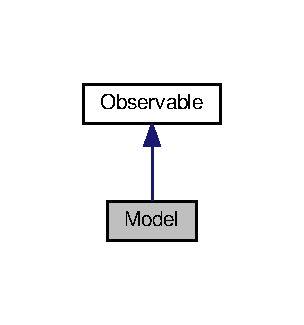
\includegraphics[width=146pt]{class_model__inherit__graph}
\end{center}
\end{figure}


Collaboration diagram for Model\-:
\nopagebreak
\begin{figure}[H]
\begin{center}
\leavevmode
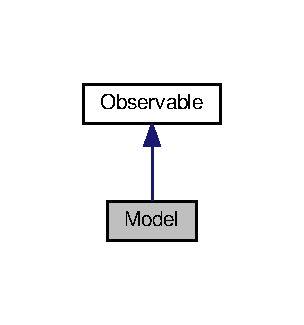
\includegraphics[width=146pt]{class_model__coll__graph}
\end{center}
\end{figure}
\subsection*{Public Member Functions}
\begin{DoxyCompactItemize}
\item 
void \hyperlink{class_model_a3484c3b12fd36cfad3a747da1f7836a6}{add\-Shape} (std\-::shared\-\_\-ptr$<$ \hyperlink{class_shape}{Shape} $>$ s)
\item 
void \hyperlink{class_model_ad606d11bbdc31559c1c31e42c739deb8}{remove\-Shape} (uint32\-\_\-t id)
\item 
void \hyperlink{class_model_a7b8102ec95ed8796b01501bf054a3330}{clear} ()
\item 
const \hyperlink{model_8h_a20f87b4e5f8cd3bd25dffa8e90e1340c}{shapes\-\_\-t} \& \hyperlink{class_model_aefac93c7d48c75209a496e24fa67b1b7}{get\-Shapes} ()
\end{DoxyCompactItemize}


\subsection{Member Function Documentation}
\hypertarget{class_model_a3484c3b12fd36cfad3a747da1f7836a6}{\index{Model@{Model}!add\-Shape@{add\-Shape}}
\index{add\-Shape@{add\-Shape}!Model@{Model}}
\subsubsection[{add\-Shape}]{\setlength{\rightskip}{0pt plus 5cm}void Model\-::add\-Shape (
\begin{DoxyParamCaption}
\item[{std\-::shared\-\_\-ptr$<$ {\bf Shape} $>$}]{s}
\end{DoxyParamCaption}
)\hspace{0.3cm}{\ttfamily [inline]}}}\label{class_model_a3484c3b12fd36cfad3a747da1f7836a6}
\hypertarget{class_model_a7b8102ec95ed8796b01501bf054a3330}{\index{Model@{Model}!clear@{clear}}
\index{clear@{clear}!Model@{Model}}
\subsubsection[{clear}]{\setlength{\rightskip}{0pt plus 5cm}void Model\-::clear (
\begin{DoxyParamCaption}
{}
\end{DoxyParamCaption}
)\hspace{0.3cm}{\ttfamily [inline]}}}\label{class_model_a7b8102ec95ed8796b01501bf054a3330}
\hypertarget{class_model_aefac93c7d48c75209a496e24fa67b1b7}{\index{Model@{Model}!get\-Shapes@{get\-Shapes}}
\index{get\-Shapes@{get\-Shapes}!Model@{Model}}
\subsubsection[{get\-Shapes}]{\setlength{\rightskip}{0pt plus 5cm}const {\bf shapes\-\_\-t}\& Model\-::get\-Shapes (
\begin{DoxyParamCaption}
{}
\end{DoxyParamCaption}
)\hspace{0.3cm}{\ttfamily [inline]}}}\label{class_model_aefac93c7d48c75209a496e24fa67b1b7}
\hypertarget{class_model_ad606d11bbdc31559c1c31e42c739deb8}{\index{Model@{Model}!remove\-Shape@{remove\-Shape}}
\index{remove\-Shape@{remove\-Shape}!Model@{Model}}
\subsubsection[{remove\-Shape}]{\setlength{\rightskip}{0pt plus 5cm}void Model\-::remove\-Shape (
\begin{DoxyParamCaption}
\item[{uint32\-\_\-t}]{id}
\end{DoxyParamCaption}
)\hspace{0.3cm}{\ttfamily [inline]}}}\label{class_model_ad606d11bbdc31559c1c31e42c739deb8}


The documentation for this class was generated from the following file\-:\begin{DoxyCompactItemize}
\item 
src/include/\hyperlink{model_8h}{model.\-h}\end{DoxyCompactItemize}

\hypertarget{class_observable}{\section{Observable Class Reference}
\label{class_observable}\index{Observable@{Observable}}
}


{\ttfamily \#include $<$observer.\-h$>$}



Inheritance diagram for Observable\-:
\nopagebreak
\begin{figure}[H]
\begin{center}
\leavevmode
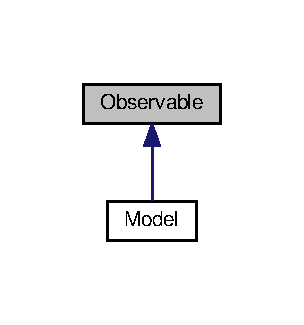
\includegraphics[width=146pt]{class_observable__inherit__graph}
\end{center}
\end{figure}
\subsection*{Public Member Functions}
\begin{DoxyCompactItemize}
\item 
void \hyperlink{class_observable_ac4c734b2866bdd881600d4fee4199d21}{add\-Observer} (\hyperlink{class_i_observer}{I\-Observer} $\ast$observer)
\item 
void \hyperlink{class_observable_a173482a397ad2669b114a424bd2fe3ac}{notify\-Update} ()
\end{DoxyCompactItemize}


\subsection{Member Function Documentation}
\hypertarget{class_observable_ac4c734b2866bdd881600d4fee4199d21}{\index{Observable@{Observable}!add\-Observer@{add\-Observer}}
\index{add\-Observer@{add\-Observer}!Observable@{Observable}}
\subsubsection[{add\-Observer}]{\setlength{\rightskip}{0pt plus 5cm}void Observable\-::add\-Observer (
\begin{DoxyParamCaption}
\item[{{\bf I\-Observer} $\ast$}]{observer}
\end{DoxyParamCaption}
)\hspace{0.3cm}{\ttfamily [inline]}}}\label{class_observable_ac4c734b2866bdd881600d4fee4199d21}
\hypertarget{class_observable_a173482a397ad2669b114a424bd2fe3ac}{\index{Observable@{Observable}!notify\-Update@{notify\-Update}}
\index{notify\-Update@{notify\-Update}!Observable@{Observable}}
\subsubsection[{notify\-Update}]{\setlength{\rightskip}{0pt plus 5cm}void Observable\-::notify\-Update (
\begin{DoxyParamCaption}
{}
\end{DoxyParamCaption}
)\hspace{0.3cm}{\ttfamily [inline]}}}\label{class_observable_a173482a397ad2669b114a424bd2fe3ac}


The documentation for this class was generated from the following file\-:\begin{DoxyCompactItemize}
\item 
src/include/\hyperlink{observer_8h}{observer.\-h}\end{DoxyCompactItemize}

\hypertarget{class_shape}{\section{Shape Class Reference}
\label{class_shape}\index{Shape@{Shape}}
}


{\ttfamily \#include $<$shape.\-h$>$}



Inheritance diagram for Shape\-:
\nopagebreak
\begin{figure}[H]
\begin{center}
\leavevmode
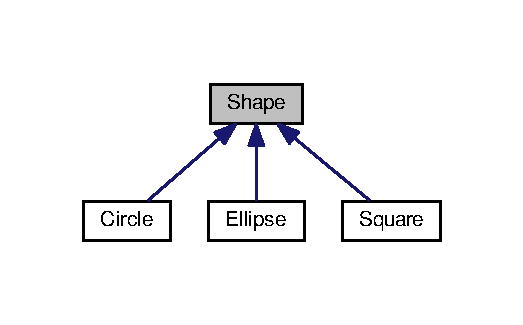
\includegraphics[width=251pt]{class_shape__inherit__graph}
\end{center}
\end{figure}
\subsection*{Public Member Functions}
\begin{DoxyCompactItemize}
\item 
\hyperlink{class_shape_aaa8d87171e65e0d8ba3c5459978992a7}{Shape} ()
\item 
uint32\-\_\-t \hyperlink{class_shape_a485401efc7beb1725c272264374f8822}{get\-Id} ()
\item 
virtual void \hyperlink{class_shape_afacc5aad8e37308c3ce8fef768199b05}{draw} ()=0
\item 
virtual std\-::string \hyperlink{class_shape_acf559a2d89e7560fbfb40a01b21f81b5}{serialize} ()
\item 
virtual void \hyperlink{class_shape_a96e9c57c68f2947ec6093c942e7f7681}{deserialize} (const std\-::string \&)
\item 
virtual \hyperlink{class_shape_ac8ad2fd02e1e94beeb98e65ab795cd56}{$\sim$\-Shape} ()=default
\end{DoxyCompactItemize}
\subsection*{Protected Attributes}
\begin{DoxyCompactItemize}
\item 
uint32\-\_\-t \hyperlink{class_shape_a5de5f48a04ef525d02a7d27b81a47c70}{\-\_\-id}
\end{DoxyCompactItemize}
\subsection*{Static Protected Attributes}
\begin{DoxyCompactItemize}
\item 
static uint32\-\_\-t \hyperlink{class_shape_ac4eb4a54d573863e093d46c707160aa5}{\-\_\-total} = 0
\end{DoxyCompactItemize}


\subsection{Constructor \& Destructor Documentation}
\hypertarget{class_shape_aaa8d87171e65e0d8ba3c5459978992a7}{\index{Shape@{Shape}!Shape@{Shape}}
\index{Shape@{Shape}!Shape@{Shape}}
\subsubsection[{Shape}]{\setlength{\rightskip}{0pt plus 5cm}Shape\-::\-Shape (
\begin{DoxyParamCaption}
{}
\end{DoxyParamCaption}
)\hspace{0.3cm}{\ttfamily [inline]}}}\label{class_shape_aaa8d87171e65e0d8ba3c5459978992a7}
\hypertarget{class_shape_ac8ad2fd02e1e94beeb98e65ab795cd56}{\index{Shape@{Shape}!$\sim$\-Shape@{$\sim$\-Shape}}
\index{$\sim$\-Shape@{$\sim$\-Shape}!Shape@{Shape}}
\subsubsection[{$\sim$\-Shape}]{\setlength{\rightskip}{0pt plus 5cm}virtual Shape\-::$\sim$\-Shape (
\begin{DoxyParamCaption}
{}
\end{DoxyParamCaption}
)\hspace{0.3cm}{\ttfamily [virtual]}, {\ttfamily [default]}}}\label{class_shape_ac8ad2fd02e1e94beeb98e65ab795cd56}


\subsection{Member Function Documentation}
\hypertarget{class_shape_a96e9c57c68f2947ec6093c942e7f7681}{\index{Shape@{Shape}!deserialize@{deserialize}}
\index{deserialize@{deserialize}!Shape@{Shape}}
\subsubsection[{deserialize}]{\setlength{\rightskip}{0pt plus 5cm}virtual void Shape\-::deserialize (
\begin{DoxyParamCaption}
\item[{const std\-::string \&}]{}
\end{DoxyParamCaption}
)\hspace{0.3cm}{\ttfamily [inline]}, {\ttfamily [virtual]}}}\label{class_shape_a96e9c57c68f2947ec6093c942e7f7681}
\hypertarget{class_shape_afacc5aad8e37308c3ce8fef768199b05}{\index{Shape@{Shape}!draw@{draw}}
\index{draw@{draw}!Shape@{Shape}}
\subsubsection[{draw}]{\setlength{\rightskip}{0pt plus 5cm}virtual void Shape\-::draw (
\begin{DoxyParamCaption}
{}
\end{DoxyParamCaption}
)\hspace{0.3cm}{\ttfamily [pure virtual]}}}\label{class_shape_afacc5aad8e37308c3ce8fef768199b05}


Implemented in \hyperlink{class_ellipse_a312c0cf0e855dc79d37c07ec52bf202e}{Ellipse}, \hyperlink{class_square_a2a8be87e5cb58dd25a8af0f6166536b9}{Square}, and \hyperlink{class_circle_a3a3f7166e7f629e44f9044b0e537eb22}{Circle}.

\hypertarget{class_shape_a485401efc7beb1725c272264374f8822}{\index{Shape@{Shape}!get\-Id@{get\-Id}}
\index{get\-Id@{get\-Id}!Shape@{Shape}}
\subsubsection[{get\-Id}]{\setlength{\rightskip}{0pt plus 5cm}uint32\-\_\-t Shape\-::get\-Id (
\begin{DoxyParamCaption}
{}
\end{DoxyParamCaption}
)\hspace{0.3cm}{\ttfamily [inline]}}}\label{class_shape_a485401efc7beb1725c272264374f8822}
\hypertarget{class_shape_acf559a2d89e7560fbfb40a01b21f81b5}{\index{Shape@{Shape}!serialize@{serialize}}
\index{serialize@{serialize}!Shape@{Shape}}
\subsubsection[{serialize}]{\setlength{\rightskip}{0pt plus 5cm}virtual std\-::string Shape\-::serialize (
\begin{DoxyParamCaption}
{}
\end{DoxyParamCaption}
)\hspace{0.3cm}{\ttfamily [inline]}, {\ttfamily [virtual]}}}\label{class_shape_acf559a2d89e7560fbfb40a01b21f81b5}


\subsection{Member Data Documentation}
\hypertarget{class_shape_a5de5f48a04ef525d02a7d27b81a47c70}{\index{Shape@{Shape}!\-\_\-id@{\-\_\-id}}
\index{\-\_\-id@{\-\_\-id}!Shape@{Shape}}
\subsubsection[{\-\_\-id}]{\setlength{\rightskip}{0pt plus 5cm}uint32\-\_\-t Shape\-::\-\_\-id\hspace{0.3cm}{\ttfamily [protected]}}}\label{class_shape_a5de5f48a04ef525d02a7d27b81a47c70}
\hypertarget{class_shape_ac4eb4a54d573863e093d46c707160aa5}{\index{Shape@{Shape}!\-\_\-total@{\-\_\-total}}
\index{\-\_\-total@{\-\_\-total}!Shape@{Shape}}
\subsubsection[{\-\_\-total}]{\setlength{\rightskip}{0pt plus 5cm}uint32\-\_\-t Shape\-::\-\_\-total = 0\hspace{0.3cm}{\ttfamily [static]}, {\ttfamily [protected]}}}\label{class_shape_ac4eb4a54d573863e093d46c707160aa5}


The documentation for this class was generated from the following file\-:\begin{DoxyCompactItemize}
\item 
src/include/\hyperlink{shape_8h}{shape.\-h}\end{DoxyCompactItemize}

\hypertarget{class_shape_factory}{\section{Shape\-Factory Class Reference}
\label{class_shape_factory}\index{Shape\-Factory@{Shape\-Factory}}
}


{\ttfamily \#include $<$shape.\-h$>$}

\subsection*{Public Types}
\begin{DoxyCompactItemize}
\item 
using \hyperlink{class_shape_factory_a4d45cc55a23b2863725a96e922c1b6e5}{registry\-\_\-map} = std\-::unordered\-\_\-map$<$ \hyperlink{shape_8h_a3c6c49dd4d974c67346f991bc443b14b}{Shapes}, void $\ast$, \hyperlink{struct_enum_class_hash}{Enum\-Class\-Hash} $>$
\end{DoxyCompactItemize}
\subsection*{Static Public Member Functions}
\begin{DoxyCompactItemize}
\item 
static \hyperlink{class_shape_factory_a4d45cc55a23b2863725a96e922c1b6e5}{registry\-\_\-map} \& \hyperlink{class_shape_factory_a9f7601b28898cb767d3c1932b88dd3e8}{registry} ()
\item 
{\footnotesize template$<$typename... T$>$ }\\static std\-::shared\-\_\-ptr$<$ \hyperlink{class_shape}{Shape} $>$ \hyperlink{class_shape_factory_af208930b3b6cd6705bb2f4347384f928}{instantiate} (\hyperlink{shape_8h_a3c6c49dd4d974c67346f991bc443b14b}{Shapes} s, T \&\&...args)
\end{DoxyCompactItemize}


\subsection{Member Typedef Documentation}
\hypertarget{class_shape_factory_a4d45cc55a23b2863725a96e922c1b6e5}{\index{Shape\-Factory@{Shape\-Factory}!registry\-\_\-map@{registry\-\_\-map}}
\index{registry\-\_\-map@{registry\-\_\-map}!ShapeFactory@{Shape\-Factory}}
\subsubsection[{registry\-\_\-map}]{\setlength{\rightskip}{0pt plus 5cm}using {\bf Shape\-Factory\-::registry\-\_\-map} =  std\-::unordered\-\_\-map$<${\bf Shapes}, void$\ast$, {\bf Enum\-Class\-Hash}$>$}}\label{class_shape_factory_a4d45cc55a23b2863725a96e922c1b6e5}


\subsection{Member Function Documentation}
\hypertarget{class_shape_factory_af208930b3b6cd6705bb2f4347384f928}{\index{Shape\-Factory@{Shape\-Factory}!instantiate@{instantiate}}
\index{instantiate@{instantiate}!ShapeFactory@{Shape\-Factory}}
\subsubsection[{instantiate}]{\setlength{\rightskip}{0pt plus 5cm}template$<$typename... T$>$ static std\-::shared\-\_\-ptr$<${\bf Shape}$>$ Shape\-Factory\-::instantiate (
\begin{DoxyParamCaption}
\item[{{\bf Shapes}}]{s, }
\item[{T \&\&...}]{args}
\end{DoxyParamCaption}
)\hspace{0.3cm}{\ttfamily [inline]}, {\ttfamily [static]}}}\label{class_shape_factory_af208930b3b6cd6705bb2f4347384f928}
\hypertarget{class_shape_factory_a9f7601b28898cb767d3c1932b88dd3e8}{\index{Shape\-Factory@{Shape\-Factory}!registry@{registry}}
\index{registry@{registry}!ShapeFactory@{Shape\-Factory}}
\subsubsection[{registry}]{\setlength{\rightskip}{0pt plus 5cm}static {\bf registry\-\_\-map}\& Shape\-Factory\-::registry (
\begin{DoxyParamCaption}
{}
\end{DoxyParamCaption}
)\hspace{0.3cm}{\ttfamily [inline]}, {\ttfamily [static]}}}\label{class_shape_factory_a9f7601b28898cb767d3c1932b88dd3e8}


The documentation for this class was generated from the following file\-:\begin{DoxyCompactItemize}
\item 
src/include/\hyperlink{shape_8h}{shape.\-h}\end{DoxyCompactItemize}

\hypertarget{struct_shape_factory_register}{\section{Shape\-Factory\-Register Struct Reference}
\label{struct_shape_factory_register}\index{Shape\-Factory\-Register@{Shape\-Factory\-Register}}
}


{\ttfamily \#include $<$shape.\-h$>$}

\subsection*{Public Member Functions}
\begin{DoxyCompactItemize}
\item 
{\footnotesize template$<$typename T $>$ }\\\hyperlink{struct_shape_factory_register_afe57a75d42e2446d3587f11cfd7f9138}{Shape\-Factory\-Register} (\hyperlink{shape_8h_a3c6c49dd4d974c67346f991bc443b14b}{Shapes} shape, T foo)
\end{DoxyCompactItemize}


\subsection{Constructor \& Destructor Documentation}
\hypertarget{struct_shape_factory_register_afe57a75d42e2446d3587f11cfd7f9138}{\index{Shape\-Factory\-Register@{Shape\-Factory\-Register}!Shape\-Factory\-Register@{Shape\-Factory\-Register}}
\index{Shape\-Factory\-Register@{Shape\-Factory\-Register}!ShapeFactoryRegister@{Shape\-Factory\-Register}}
\subsubsection[{Shape\-Factory\-Register}]{\setlength{\rightskip}{0pt plus 5cm}template$<$typename T $>$ Shape\-Factory\-Register\-::\-Shape\-Factory\-Register (
\begin{DoxyParamCaption}
\item[{{\bf Shapes}}]{shape, }
\item[{T}]{foo}
\end{DoxyParamCaption}
)\hspace{0.3cm}{\ttfamily [inline]}}}\label{struct_shape_factory_register_afe57a75d42e2446d3587f11cfd7f9138}


The documentation for this struct was generated from the following file\-:\begin{DoxyCompactItemize}
\item 
src/include/\hyperlink{shape_8h}{shape.\-h}\end{DoxyCompactItemize}

\hypertarget{class_square}{\section{Square Class Reference}
\label{class_square}\index{Square@{Square}}
}


{\ttfamily \#include $<$shape.\-h$>$}



Inheritance diagram for Square\-:
\nopagebreak
\begin{figure}[H]
\begin{center}
\leavevmode
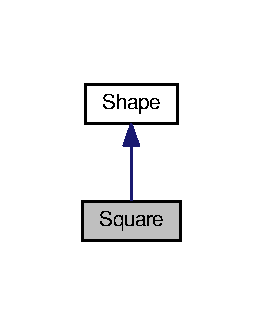
\includegraphics[width=126pt]{class_square__inherit__graph}
\end{center}
\end{figure}


Collaboration diagram for Square\-:
\nopagebreak
\begin{figure}[H]
\begin{center}
\leavevmode
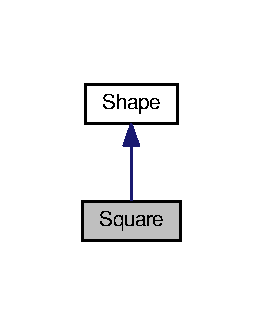
\includegraphics[width=126pt]{class_square__coll__graph}
\end{center}
\end{figure}
\subsection*{Public Member Functions}
\begin{DoxyCompactItemize}
\item 
\hyperlink{class_square_afd27b0650fb7baa1dacb2a452aba121e}{Square} (uint32\-\_\-t x1, uint32\-\_\-t y1, uint32\-\_\-t x2, uint32\-\_\-t y2)
\item 
void \hyperlink{class_square_a2a8be87e5cb58dd25a8af0f6166536b9}{draw} ()
\end{DoxyCompactItemize}
\subsection*{Static Public Member Functions}
\begin{DoxyCompactItemize}
\item 
static std\-::shared\-\_\-ptr$<$ \hyperlink{class_shape}{Shape} $>$ \hyperlink{class_square_aa9a44b475f029c4dda064bf9fed49700}{create} (uint32\-\_\-t x1, uint32\-\_\-t y1, uint32\-\_\-t x2, uint32\-\_\-t y2)
\end{DoxyCompactItemize}
\subsection*{Additional Inherited Members}


\subsection{Constructor \& Destructor Documentation}
\hypertarget{class_square_afd27b0650fb7baa1dacb2a452aba121e}{\index{Square@{Square}!Square@{Square}}
\index{Square@{Square}!Square@{Square}}
\subsubsection[{Square}]{\setlength{\rightskip}{0pt plus 5cm}Square\-::\-Square (
\begin{DoxyParamCaption}
\item[{uint32\-\_\-t}]{x1, }
\item[{uint32\-\_\-t}]{y1, }
\item[{uint32\-\_\-t}]{x2, }
\item[{uint32\-\_\-t}]{y2}
\end{DoxyParamCaption}
)\hspace{0.3cm}{\ttfamily [inline]}}}\label{class_square_afd27b0650fb7baa1dacb2a452aba121e}


\subsection{Member Function Documentation}
\hypertarget{class_square_aa9a44b475f029c4dda064bf9fed49700}{\index{Square@{Square}!create@{create}}
\index{create@{create}!Square@{Square}}
\subsubsection[{create}]{\setlength{\rightskip}{0pt plus 5cm}static std\-::shared\-\_\-ptr$<${\bf Shape}$>$ Square\-::create (
\begin{DoxyParamCaption}
\item[{uint32\-\_\-t}]{x1, }
\item[{uint32\-\_\-t}]{y1, }
\item[{uint32\-\_\-t}]{x2, }
\item[{uint32\-\_\-t}]{y2}
\end{DoxyParamCaption}
)\hspace{0.3cm}{\ttfamily [inline]}, {\ttfamily [static]}}}\label{class_square_aa9a44b475f029c4dda064bf9fed49700}
\hypertarget{class_square_a2a8be87e5cb58dd25a8af0f6166536b9}{\index{Square@{Square}!draw@{draw}}
\index{draw@{draw}!Square@{Square}}
\subsubsection[{draw}]{\setlength{\rightskip}{0pt plus 5cm}void Square\-::draw (
\begin{DoxyParamCaption}
{}
\end{DoxyParamCaption}
)\hspace{0.3cm}{\ttfamily [inline]}, {\ttfamily [virtual]}}}\label{class_square_a2a8be87e5cb58dd25a8af0f6166536b9}


Implements \hyperlink{class_shape_afacc5aad8e37308c3ce8fef768199b05}{Shape}.



The documentation for this class was generated from the following file\-:\begin{DoxyCompactItemize}
\item 
src/include/\hyperlink{shape_8h}{shape.\-h}\end{DoxyCompactItemize}

\hypertarget{class_view}{\section{View Class Reference}
\label{class_view}\index{View@{View}}
}


{\ttfamily \#include $<$view.\-h$>$}



Inheritance diagram for View\-:
\nopagebreak
\begin{figure}[H]
\begin{center}
\leavevmode
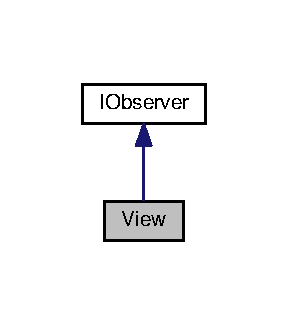
\includegraphics[width=138pt]{class_view__inherit__graph}
\end{center}
\end{figure}


Collaboration diagram for View\-:
\nopagebreak
\begin{figure}[H]
\begin{center}
\leavevmode
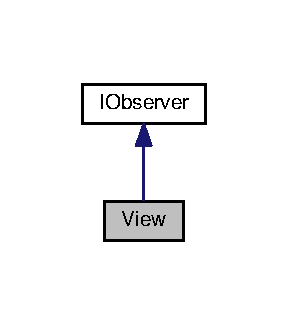
\includegraphics[width=138pt]{class_view__coll__graph}
\end{center}
\end{figure}
\subsection*{Public Member Functions}
\begin{DoxyCompactItemize}
\item 
\hyperlink{class_view_a44ad60a768422d3fa8fbd7576950080a}{View} ()
\item 
\hyperlink{class_view_a9b238149eafd4bb390ca043437e2b5e8}{View} (std\-::shared\-\_\-ptr$<$ \hyperlink{class_model}{Model} $>$ model)
\item 
void \hyperlink{class_view_aae801a3576c7b6c236ede6d4d6717c06}{set\-Model} (std\-::shared\-\_\-ptr$<$ \hyperlink{class_model}{Model} $>$ model)
\item 
void \hyperlink{class_view_a1c98202846728b495760fad0907b8b0f}{update} ()
\end{DoxyCompactItemize}


\subsection{Constructor \& Destructor Documentation}
\hypertarget{class_view_a44ad60a768422d3fa8fbd7576950080a}{\index{View@{View}!View@{View}}
\index{View@{View}!View@{View}}
\subsubsection[{View}]{\setlength{\rightskip}{0pt plus 5cm}View\-::\-View (
\begin{DoxyParamCaption}
{}
\end{DoxyParamCaption}
)\hspace{0.3cm}{\ttfamily [inline]}}}\label{class_view_a44ad60a768422d3fa8fbd7576950080a}
\hypertarget{class_view_a9b238149eafd4bb390ca043437e2b5e8}{\index{View@{View}!View@{View}}
\index{View@{View}!View@{View}}
\subsubsection[{View}]{\setlength{\rightskip}{0pt plus 5cm}View\-::\-View (
\begin{DoxyParamCaption}
\item[{std\-::shared\-\_\-ptr$<$ {\bf Model} $>$}]{model}
\end{DoxyParamCaption}
)\hspace{0.3cm}{\ttfamily [inline]}}}\label{class_view_a9b238149eafd4bb390ca043437e2b5e8}


\subsection{Member Function Documentation}
\hypertarget{class_view_aae801a3576c7b6c236ede6d4d6717c06}{\index{View@{View}!set\-Model@{set\-Model}}
\index{set\-Model@{set\-Model}!View@{View}}
\subsubsection[{set\-Model}]{\setlength{\rightskip}{0pt plus 5cm}void View\-::set\-Model (
\begin{DoxyParamCaption}
\item[{std\-::shared\-\_\-ptr$<$ {\bf Model} $>$}]{model}
\end{DoxyParamCaption}
)\hspace{0.3cm}{\ttfamily [inline]}}}\label{class_view_aae801a3576c7b6c236ede6d4d6717c06}
\hypertarget{class_view_a1c98202846728b495760fad0907b8b0f}{\index{View@{View}!update@{update}}
\index{update@{update}!View@{View}}
\subsubsection[{update}]{\setlength{\rightskip}{0pt plus 5cm}void View\-::update (
\begin{DoxyParamCaption}
{}
\end{DoxyParamCaption}
)\hspace{0.3cm}{\ttfamily [inline]}, {\ttfamily [virtual]}}}\label{class_view_a1c98202846728b495760fad0907b8b0f}


Implements \hyperlink{class_i_observer_a91a4770cbec97439f2faba69a1ed72e0}{I\-Observer}.



The documentation for this class was generated from the following file\-:\begin{DoxyCompactItemize}
\item 
src/include/\hyperlink{view_8h}{view.\-h}\end{DoxyCompactItemize}

\chapter{File Documentation}
\hypertarget{_c_make_c_compiler_id_8c}{\section{C\-Make\-Files/3.9.2/\-Compiler\-Id\-C/\-C\-Make\-C\-Compiler\-Id.c File Reference}
\label{_c_make_c_compiler_id_8c}\index{C\-Make\-Files/3.\-9.\-2/\-Compiler\-Id\-C/\-C\-Make\-C\-Compiler\-Id.\-c@{C\-Make\-Files/3.\-9.\-2/\-Compiler\-Id\-C/\-C\-Make\-C\-Compiler\-Id.\-c}}
}
\subsection*{Macros}
\begin{DoxyCompactItemize}
\item 
\#define \hyperlink{_c_make_c_compiler_id_8c_a81dee0709ded976b2e0319239f72d174}{C\-O\-M\-P\-I\-L\-E\-R\-\_\-\-I\-D}~\char`\"{}\char`\"{}
\item 
\#define \hyperlink{_c_make_c_compiler_id_8c_a2ae9b72bb13abaabfcf2ee0ba7d3fa1d}{S\-T\-R\-I\-N\-G\-I\-F\-Y\-\_\-\-H\-E\-L\-P\-E\-R}(X)~\#X
\item 
\#define \hyperlink{_c_make_c_compiler_id_8c_a43e1cad902b6477bec893cb6430bd6c8}{S\-T\-R\-I\-N\-G\-I\-F\-Y}(X)~\hyperlink{_c_make_c_x_x_compiler_id_8cpp_a2ae9b72bb13abaabfcf2ee0ba7d3fa1d}{S\-T\-R\-I\-N\-G\-I\-F\-Y\-\_\-\-H\-E\-L\-P\-E\-R}(X)
\item 
\#define \hyperlink{_c_make_c_compiler_id_8c_adbc5372f40838899018fadbc89bd588b}{P\-L\-A\-T\-F\-O\-R\-M\-\_\-\-I\-D}
\item 
\#define \hyperlink{_c_make_c_compiler_id_8c_aba35d0d200deaeb06aee95ca297acb28}{A\-R\-C\-H\-I\-T\-E\-C\-T\-U\-R\-E\-\_\-\-I\-D}
\item 
\#define \hyperlink{_c_make_c_compiler_id_8c_ad1280362da42492bbc11aa78cbf776ad}{D\-E\-C}(n)
\item 
\#define \hyperlink{_c_make_c_compiler_id_8c_a46d5d95daa1bef867bd0179594310ed5}{H\-E\-X}(n)
\item 
\#define \hyperlink{_c_make_c_compiler_id_8c_a07f8e5783674099cd7f5110e22a78cdb}{C\-\_\-\-D\-I\-A\-L\-E\-C\-T}
\end{DoxyCompactItemize}
\subsection*{Functions}
\begin{DoxyCompactItemize}
\item 
int \hyperlink{_c_make_c_compiler_id_8c_a0ddf1224851353fc92bfbff6f499fa97}{main} (int argc, char $\ast$argv\mbox{[}$\,$\mbox{]})
\end{DoxyCompactItemize}
\subsection*{Variables}
\begin{DoxyCompactItemize}
\item 
char const $\ast$ \hyperlink{_c_make_c_compiler_id_8c_a4b0efeb7a5d59313986b3a0390f050f6}{info\-\_\-compiler} = \char`\"{}I\-N\-F\-O\char`\"{} \char`\"{}\-:\char`\"{} \char`\"{}compiler\mbox{[}\char`\"{} C\-O\-M\-P\-I\-L\-E\-R\-\_\-\-I\-D \char`\"{}\mbox{]}\char`\"{}
\item 
char const $\ast$ \hyperlink{_c_make_c_compiler_id_8c_a2321403dee54ee23f0c2fa849c60f7d4}{info\-\_\-platform} = \char`\"{}I\-N\-F\-O\char`\"{} \char`\"{}\-:\char`\"{} \char`\"{}platform\mbox{[}\char`\"{} P\-L\-A\-T\-F\-O\-R\-M\-\_\-\-I\-D \char`\"{}\mbox{]}\char`\"{}
\item 
char const $\ast$ \hyperlink{_c_make_c_compiler_id_8c_a59647e99d304ed33b15cb284c27ed391}{info\-\_\-arch} = \char`\"{}I\-N\-F\-O\char`\"{} \char`\"{}\-:\char`\"{} \char`\"{}arch\mbox{[}\char`\"{} A\-R\-C\-H\-I\-T\-E\-C\-T\-U\-R\-E\-\_\-\-I\-D \char`\"{}\mbox{]}\char`\"{}
\item 
const char $\ast$ \hyperlink{_c_make_c_compiler_id_8c_a1ce162bad2fe6966ac8b33cc19e120b8}{info\-\_\-language\-\_\-dialect\-\_\-default}
\end{DoxyCompactItemize}


\subsection{Macro Definition Documentation}
\hypertarget{_c_make_c_compiler_id_8c_aba35d0d200deaeb06aee95ca297acb28}{\index{C\-Make\-C\-Compiler\-Id.\-c@{C\-Make\-C\-Compiler\-Id.\-c}!A\-R\-C\-H\-I\-T\-E\-C\-T\-U\-R\-E\-\_\-\-I\-D@{A\-R\-C\-H\-I\-T\-E\-C\-T\-U\-R\-E\-\_\-\-I\-D}}
\index{A\-R\-C\-H\-I\-T\-E\-C\-T\-U\-R\-E\-\_\-\-I\-D@{A\-R\-C\-H\-I\-T\-E\-C\-T\-U\-R\-E\-\_\-\-I\-D}!CMakeCCompilerId.c@{C\-Make\-C\-Compiler\-Id.\-c}}
\subsubsection[{A\-R\-C\-H\-I\-T\-E\-C\-T\-U\-R\-E\-\_\-\-I\-D}]{\setlength{\rightskip}{0pt plus 5cm}\#define A\-R\-C\-H\-I\-T\-E\-C\-T\-U\-R\-E\-\_\-\-I\-D}}\label{_c_make_c_compiler_id_8c_aba35d0d200deaeb06aee95ca297acb28}
\hypertarget{_c_make_c_compiler_id_8c_a07f8e5783674099cd7f5110e22a78cdb}{\index{C\-Make\-C\-Compiler\-Id.\-c@{C\-Make\-C\-Compiler\-Id.\-c}!C\-\_\-\-D\-I\-A\-L\-E\-C\-T@{C\-\_\-\-D\-I\-A\-L\-E\-C\-T}}
\index{C\-\_\-\-D\-I\-A\-L\-E\-C\-T@{C\-\_\-\-D\-I\-A\-L\-E\-C\-T}!CMakeCCompilerId.c@{C\-Make\-C\-Compiler\-Id.\-c}}
\subsubsection[{C\-\_\-\-D\-I\-A\-L\-E\-C\-T}]{\setlength{\rightskip}{0pt plus 5cm}\#define C\-\_\-\-D\-I\-A\-L\-E\-C\-T}}\label{_c_make_c_compiler_id_8c_a07f8e5783674099cd7f5110e22a78cdb}
\hypertarget{_c_make_c_compiler_id_8c_a81dee0709ded976b2e0319239f72d174}{\index{C\-Make\-C\-Compiler\-Id.\-c@{C\-Make\-C\-Compiler\-Id.\-c}!C\-O\-M\-P\-I\-L\-E\-R\-\_\-\-I\-D@{C\-O\-M\-P\-I\-L\-E\-R\-\_\-\-I\-D}}
\index{C\-O\-M\-P\-I\-L\-E\-R\-\_\-\-I\-D@{C\-O\-M\-P\-I\-L\-E\-R\-\_\-\-I\-D}!CMakeCCompilerId.c@{C\-Make\-C\-Compiler\-Id.\-c}}
\subsubsection[{C\-O\-M\-P\-I\-L\-E\-R\-\_\-\-I\-D}]{\setlength{\rightskip}{0pt plus 5cm}\#define C\-O\-M\-P\-I\-L\-E\-R\-\_\-\-I\-D~\char`\"{}\char`\"{}}}\label{_c_make_c_compiler_id_8c_a81dee0709ded976b2e0319239f72d174}
\hypertarget{_c_make_c_compiler_id_8c_ad1280362da42492bbc11aa78cbf776ad}{\index{C\-Make\-C\-Compiler\-Id.\-c@{C\-Make\-C\-Compiler\-Id.\-c}!D\-E\-C@{D\-E\-C}}
\index{D\-E\-C@{D\-E\-C}!CMakeCCompilerId.c@{C\-Make\-C\-Compiler\-Id.\-c}}
\subsubsection[{D\-E\-C}]{\setlength{\rightskip}{0pt plus 5cm}\#define D\-E\-C(
\begin{DoxyParamCaption}
\item[{}]{n}
\end{DoxyParamCaption}
)}}\label{_c_make_c_compiler_id_8c_ad1280362da42492bbc11aa78cbf776ad}
{\bfseries Value\-:}
\begin{DoxyCode}
(\textcolor{charliteral}{'0'} + (((n) / 10000000)%10)), \(\backslash\)
  (\textcolor{charliteral}{'0'} + (((n) / 1000000)%10)),  \(\backslash\)
  (\textcolor{charliteral}{'0'} + (((n) / 100000)%10)),   \(\backslash\)
  (\textcolor{charliteral}{'0'} + (((n) / 10000)%10)),    \(\backslash\)
  (\textcolor{charliteral}{'0'} + (((n) / 1000)%10)),     \(\backslash\)
  (\textcolor{charliteral}{'0'} + (((n) / 100)%10)),      \(\backslash\)
  (\textcolor{charliteral}{'0'} + (((n) / 10)%10)),       \(\backslash\)
  (\textcolor{charliteral}{'0'} +  ((n) % 10))
\end{DoxyCode}
\hypertarget{_c_make_c_compiler_id_8c_a46d5d95daa1bef867bd0179594310ed5}{\index{C\-Make\-C\-Compiler\-Id.\-c@{C\-Make\-C\-Compiler\-Id.\-c}!H\-E\-X@{H\-E\-X}}
\index{H\-E\-X@{H\-E\-X}!CMakeCCompilerId.c@{C\-Make\-C\-Compiler\-Id.\-c}}
\subsubsection[{H\-E\-X}]{\setlength{\rightskip}{0pt plus 5cm}\#define H\-E\-X(
\begin{DoxyParamCaption}
\item[{}]{n}
\end{DoxyParamCaption}
)}}\label{_c_make_c_compiler_id_8c_a46d5d95daa1bef867bd0179594310ed5}
{\bfseries Value\-:}
\begin{DoxyCode}
(\textcolor{charliteral}{'0'} + ((n)>>28 & 0xF)), \(\backslash\)
  (\textcolor{charliteral}{'0'} + ((n)>>24 & 0xF)), \(\backslash\)
  (\textcolor{charliteral}{'0'} + ((n)>>20 & 0xF)), \(\backslash\)
  (\textcolor{charliteral}{'0'} + ((n)>>16 & 0xF)), \(\backslash\)
  (\textcolor{charliteral}{'0'} + ((n)>>12 & 0xF)), \(\backslash\)
  (\textcolor{charliteral}{'0'} + ((n)>>8  & 0xF)), \(\backslash\)
  (\textcolor{charliteral}{'0'} + ((n)>>4  & 0xF)), \(\backslash\)
  (\textcolor{charliteral}{'0'} + ((n)     & 0xF))
\end{DoxyCode}
\hypertarget{_c_make_c_compiler_id_8c_adbc5372f40838899018fadbc89bd588b}{\index{C\-Make\-C\-Compiler\-Id.\-c@{C\-Make\-C\-Compiler\-Id.\-c}!P\-L\-A\-T\-F\-O\-R\-M\-\_\-\-I\-D@{P\-L\-A\-T\-F\-O\-R\-M\-\_\-\-I\-D}}
\index{P\-L\-A\-T\-F\-O\-R\-M\-\_\-\-I\-D@{P\-L\-A\-T\-F\-O\-R\-M\-\_\-\-I\-D}!CMakeCCompilerId.c@{C\-Make\-C\-Compiler\-Id.\-c}}
\subsubsection[{P\-L\-A\-T\-F\-O\-R\-M\-\_\-\-I\-D}]{\setlength{\rightskip}{0pt plus 5cm}\#define P\-L\-A\-T\-F\-O\-R\-M\-\_\-\-I\-D}}\label{_c_make_c_compiler_id_8c_adbc5372f40838899018fadbc89bd588b}
\hypertarget{_c_make_c_compiler_id_8c_a43e1cad902b6477bec893cb6430bd6c8}{\index{C\-Make\-C\-Compiler\-Id.\-c@{C\-Make\-C\-Compiler\-Id.\-c}!S\-T\-R\-I\-N\-G\-I\-F\-Y@{S\-T\-R\-I\-N\-G\-I\-F\-Y}}
\index{S\-T\-R\-I\-N\-G\-I\-F\-Y@{S\-T\-R\-I\-N\-G\-I\-F\-Y}!CMakeCCompilerId.c@{C\-Make\-C\-Compiler\-Id.\-c}}
\subsubsection[{S\-T\-R\-I\-N\-G\-I\-F\-Y}]{\setlength{\rightskip}{0pt plus 5cm}\#define S\-T\-R\-I\-N\-G\-I\-F\-Y(
\begin{DoxyParamCaption}
\item[{}]{X}
\end{DoxyParamCaption}
)~{\bf S\-T\-R\-I\-N\-G\-I\-F\-Y\-\_\-\-H\-E\-L\-P\-E\-R}(X)}}\label{_c_make_c_compiler_id_8c_a43e1cad902b6477bec893cb6430bd6c8}
\hypertarget{_c_make_c_compiler_id_8c_a2ae9b72bb13abaabfcf2ee0ba7d3fa1d}{\index{C\-Make\-C\-Compiler\-Id.\-c@{C\-Make\-C\-Compiler\-Id.\-c}!S\-T\-R\-I\-N\-G\-I\-F\-Y\-\_\-\-H\-E\-L\-P\-E\-R@{S\-T\-R\-I\-N\-G\-I\-F\-Y\-\_\-\-H\-E\-L\-P\-E\-R}}
\index{S\-T\-R\-I\-N\-G\-I\-F\-Y\-\_\-\-H\-E\-L\-P\-E\-R@{S\-T\-R\-I\-N\-G\-I\-F\-Y\-\_\-\-H\-E\-L\-P\-E\-R}!CMakeCCompilerId.c@{C\-Make\-C\-Compiler\-Id.\-c}}
\subsubsection[{S\-T\-R\-I\-N\-G\-I\-F\-Y\-\_\-\-H\-E\-L\-P\-E\-R}]{\setlength{\rightskip}{0pt plus 5cm}\#define S\-T\-R\-I\-N\-G\-I\-F\-Y\-\_\-\-H\-E\-L\-P\-E\-R(
\begin{DoxyParamCaption}
\item[{}]{X}
\end{DoxyParamCaption}
)~\#X}}\label{_c_make_c_compiler_id_8c_a2ae9b72bb13abaabfcf2ee0ba7d3fa1d}


\subsection{Function Documentation}
\hypertarget{_c_make_c_compiler_id_8c_a0ddf1224851353fc92bfbff6f499fa97}{\index{C\-Make\-C\-Compiler\-Id.\-c@{C\-Make\-C\-Compiler\-Id.\-c}!main@{main}}
\index{main@{main}!CMakeCCompilerId.c@{C\-Make\-C\-Compiler\-Id.\-c}}
\subsubsection[{main}]{\setlength{\rightskip}{0pt plus 5cm}int main (
\begin{DoxyParamCaption}
\item[{int}]{argc, }
\item[{char $\ast$}]{argv\mbox{[}$\,$\mbox{]}}
\end{DoxyParamCaption}
)}}\label{_c_make_c_compiler_id_8c_a0ddf1224851353fc92bfbff6f499fa97}


\subsection{Variable Documentation}
\hypertarget{_c_make_c_compiler_id_8c_a59647e99d304ed33b15cb284c27ed391}{\index{C\-Make\-C\-Compiler\-Id.\-c@{C\-Make\-C\-Compiler\-Id.\-c}!info\-\_\-arch@{info\-\_\-arch}}
\index{info\-\_\-arch@{info\-\_\-arch}!CMakeCCompilerId.c@{C\-Make\-C\-Compiler\-Id.\-c}}
\subsubsection[{info\-\_\-arch}]{\setlength{\rightskip}{0pt plus 5cm}char const$\ast$ info\-\_\-arch = \char`\"{}I\-N\-F\-O\char`\"{} \char`\"{}\-:\char`\"{} \char`\"{}arch\mbox{[}\char`\"{} A\-R\-C\-H\-I\-T\-E\-C\-T\-U\-R\-E\-\_\-\-I\-D \char`\"{}\mbox{]}\char`\"{}}}\label{_c_make_c_compiler_id_8c_a59647e99d304ed33b15cb284c27ed391}
\hypertarget{_c_make_c_compiler_id_8c_a4b0efeb7a5d59313986b3a0390f050f6}{\index{C\-Make\-C\-Compiler\-Id.\-c@{C\-Make\-C\-Compiler\-Id.\-c}!info\-\_\-compiler@{info\-\_\-compiler}}
\index{info\-\_\-compiler@{info\-\_\-compiler}!CMakeCCompilerId.c@{C\-Make\-C\-Compiler\-Id.\-c}}
\subsubsection[{info\-\_\-compiler}]{\setlength{\rightskip}{0pt plus 5cm}char const$\ast$ info\-\_\-compiler = \char`\"{}I\-N\-F\-O\char`\"{} \char`\"{}\-:\char`\"{} \char`\"{}compiler\mbox{[}\char`\"{} C\-O\-M\-P\-I\-L\-E\-R\-\_\-\-I\-D \char`\"{}\mbox{]}\char`\"{}}}\label{_c_make_c_compiler_id_8c_a4b0efeb7a5d59313986b3a0390f050f6}
\hypertarget{_c_make_c_compiler_id_8c_a1ce162bad2fe6966ac8b33cc19e120b8}{\index{C\-Make\-C\-Compiler\-Id.\-c@{C\-Make\-C\-Compiler\-Id.\-c}!info\-\_\-language\-\_\-dialect\-\_\-default@{info\-\_\-language\-\_\-dialect\-\_\-default}}
\index{info\-\_\-language\-\_\-dialect\-\_\-default@{info\-\_\-language\-\_\-dialect\-\_\-default}!CMakeCCompilerId.c@{C\-Make\-C\-Compiler\-Id.\-c}}
\subsubsection[{info\-\_\-language\-\_\-dialect\-\_\-default}]{\setlength{\rightskip}{0pt plus 5cm}const char$\ast$ info\-\_\-language\-\_\-dialect\-\_\-default}}\label{_c_make_c_compiler_id_8c_a1ce162bad2fe6966ac8b33cc19e120b8}
{\bfseries Initial value\-:}
\begin{DoxyCode}
=
  \textcolor{stringliteral}{"INFO"} \textcolor{stringliteral}{":"} \textcolor{stringliteral}{"dialect\_default["} \hyperlink{_c_make_c_compiler_id_8c_a07f8e5783674099cd7f5110e22a78cdb}{C\_DIALECT} \textcolor{stringliteral}{"]"}
\end{DoxyCode}
\hypertarget{_c_make_c_compiler_id_8c_a2321403dee54ee23f0c2fa849c60f7d4}{\index{C\-Make\-C\-Compiler\-Id.\-c@{C\-Make\-C\-Compiler\-Id.\-c}!info\-\_\-platform@{info\-\_\-platform}}
\index{info\-\_\-platform@{info\-\_\-platform}!CMakeCCompilerId.c@{C\-Make\-C\-Compiler\-Id.\-c}}
\subsubsection[{info\-\_\-platform}]{\setlength{\rightskip}{0pt plus 5cm}char const$\ast$ info\-\_\-platform = \char`\"{}I\-N\-F\-O\char`\"{} \char`\"{}\-:\char`\"{} \char`\"{}platform\mbox{[}\char`\"{} P\-L\-A\-T\-F\-O\-R\-M\-\_\-\-I\-D \char`\"{}\mbox{]}\char`\"{}}}\label{_c_make_c_compiler_id_8c_a2321403dee54ee23f0c2fa849c60f7d4}

\hypertarget{_c_make_c_x_x_compiler_id_8cpp}{\section{C\-Make\-Files/3.9.2/\-Compiler\-Id\-C\-X\-X/\-C\-Make\-C\-X\-X\-Compiler\-Id.cpp File Reference}
\label{_c_make_c_x_x_compiler_id_8cpp}\index{C\-Make\-Files/3.\-9.\-2/\-Compiler\-Id\-C\-X\-X/\-C\-Make\-C\-X\-X\-Compiler\-Id.\-cpp@{C\-Make\-Files/3.\-9.\-2/\-Compiler\-Id\-C\-X\-X/\-C\-Make\-C\-X\-X\-Compiler\-Id.\-cpp}}
}
\subsection*{Macros}
\begin{DoxyCompactItemize}
\item 
\#define \hyperlink{_c_make_c_x_x_compiler_id_8cpp_a81dee0709ded976b2e0319239f72d174}{C\-O\-M\-P\-I\-L\-E\-R\-\_\-\-I\-D}~\char`\"{}\char`\"{}
\item 
\#define \hyperlink{_c_make_c_x_x_compiler_id_8cpp_a2ae9b72bb13abaabfcf2ee0ba7d3fa1d}{S\-T\-R\-I\-N\-G\-I\-F\-Y\-\_\-\-H\-E\-L\-P\-E\-R}(X)~\#X
\item 
\#define \hyperlink{_c_make_c_x_x_compiler_id_8cpp_a43e1cad902b6477bec893cb6430bd6c8}{S\-T\-R\-I\-N\-G\-I\-F\-Y}(X)~\hyperlink{_c_make_c_x_x_compiler_id_8cpp_a2ae9b72bb13abaabfcf2ee0ba7d3fa1d}{S\-T\-R\-I\-N\-G\-I\-F\-Y\-\_\-\-H\-E\-L\-P\-E\-R}(X)
\item 
\#define \hyperlink{_c_make_c_x_x_compiler_id_8cpp_adbc5372f40838899018fadbc89bd588b}{P\-L\-A\-T\-F\-O\-R\-M\-\_\-\-I\-D}
\item 
\#define \hyperlink{_c_make_c_x_x_compiler_id_8cpp_aba35d0d200deaeb06aee95ca297acb28}{A\-R\-C\-H\-I\-T\-E\-C\-T\-U\-R\-E\-\_\-\-I\-D}
\item 
\#define \hyperlink{_c_make_c_x_x_compiler_id_8cpp_ad1280362da42492bbc11aa78cbf776ad}{D\-E\-C}(n)
\item 
\#define \hyperlink{_c_make_c_x_x_compiler_id_8cpp_a46d5d95daa1bef867bd0179594310ed5}{H\-E\-X}(n)
\end{DoxyCompactItemize}
\subsection*{Functions}
\begin{DoxyCompactItemize}
\item 
int \hyperlink{_c_make_c_x_x_compiler_id_8cpp_a0ddf1224851353fc92bfbff6f499fa97}{main} (int argc, char $\ast$argv\mbox{[}$\,$\mbox{]})
\end{DoxyCompactItemize}
\subsection*{Variables}
\begin{DoxyCompactItemize}
\item 
char const $\ast$ \hyperlink{_c_make_c_x_x_compiler_id_8cpp_a4b0efeb7a5d59313986b3a0390f050f6}{info\-\_\-compiler} = \char`\"{}I\-N\-F\-O\char`\"{} \char`\"{}\-:\char`\"{} \char`\"{}compiler\mbox{[}\char`\"{} C\-O\-M\-P\-I\-L\-E\-R\-\_\-\-I\-D \char`\"{}\mbox{]}\char`\"{}
\item 
char const $\ast$ \hyperlink{_c_make_c_x_x_compiler_id_8cpp_a2321403dee54ee23f0c2fa849c60f7d4}{info\-\_\-platform} = \char`\"{}I\-N\-F\-O\char`\"{} \char`\"{}\-:\char`\"{} \char`\"{}platform\mbox{[}\char`\"{} P\-L\-A\-T\-F\-O\-R\-M\-\_\-\-I\-D \char`\"{}\mbox{]}\char`\"{}
\item 
char const $\ast$ \hyperlink{_c_make_c_x_x_compiler_id_8cpp_a59647e99d304ed33b15cb284c27ed391}{info\-\_\-arch} = \char`\"{}I\-N\-F\-O\char`\"{} \char`\"{}\-:\char`\"{} \char`\"{}arch\mbox{[}\char`\"{} A\-R\-C\-H\-I\-T\-E\-C\-T\-U\-R\-E\-\_\-\-I\-D \char`\"{}\mbox{]}\char`\"{}
\item 
const char $\ast$ \hyperlink{_c_make_c_x_x_compiler_id_8cpp_a1ce162bad2fe6966ac8b33cc19e120b8}{info\-\_\-language\-\_\-dialect\-\_\-default}
\end{DoxyCompactItemize}


\subsection{Macro Definition Documentation}
\hypertarget{_c_make_c_x_x_compiler_id_8cpp_aba35d0d200deaeb06aee95ca297acb28}{\index{C\-Make\-C\-X\-X\-Compiler\-Id.\-cpp@{C\-Make\-C\-X\-X\-Compiler\-Id.\-cpp}!A\-R\-C\-H\-I\-T\-E\-C\-T\-U\-R\-E\-\_\-\-I\-D@{A\-R\-C\-H\-I\-T\-E\-C\-T\-U\-R\-E\-\_\-\-I\-D}}
\index{A\-R\-C\-H\-I\-T\-E\-C\-T\-U\-R\-E\-\_\-\-I\-D@{A\-R\-C\-H\-I\-T\-E\-C\-T\-U\-R\-E\-\_\-\-I\-D}!CMakeCXXCompilerId.cpp@{C\-Make\-C\-X\-X\-Compiler\-Id.\-cpp}}
\subsubsection[{A\-R\-C\-H\-I\-T\-E\-C\-T\-U\-R\-E\-\_\-\-I\-D}]{\setlength{\rightskip}{0pt plus 5cm}\#define A\-R\-C\-H\-I\-T\-E\-C\-T\-U\-R\-E\-\_\-\-I\-D}}\label{_c_make_c_x_x_compiler_id_8cpp_aba35d0d200deaeb06aee95ca297acb28}
\hypertarget{_c_make_c_x_x_compiler_id_8cpp_a81dee0709ded976b2e0319239f72d174}{\index{C\-Make\-C\-X\-X\-Compiler\-Id.\-cpp@{C\-Make\-C\-X\-X\-Compiler\-Id.\-cpp}!C\-O\-M\-P\-I\-L\-E\-R\-\_\-\-I\-D@{C\-O\-M\-P\-I\-L\-E\-R\-\_\-\-I\-D}}
\index{C\-O\-M\-P\-I\-L\-E\-R\-\_\-\-I\-D@{C\-O\-M\-P\-I\-L\-E\-R\-\_\-\-I\-D}!CMakeCXXCompilerId.cpp@{C\-Make\-C\-X\-X\-Compiler\-Id.\-cpp}}
\subsubsection[{C\-O\-M\-P\-I\-L\-E\-R\-\_\-\-I\-D}]{\setlength{\rightskip}{0pt plus 5cm}\#define C\-O\-M\-P\-I\-L\-E\-R\-\_\-\-I\-D~\char`\"{}\char`\"{}}}\label{_c_make_c_x_x_compiler_id_8cpp_a81dee0709ded976b2e0319239f72d174}
\hypertarget{_c_make_c_x_x_compiler_id_8cpp_ad1280362da42492bbc11aa78cbf776ad}{\index{C\-Make\-C\-X\-X\-Compiler\-Id.\-cpp@{C\-Make\-C\-X\-X\-Compiler\-Id.\-cpp}!D\-E\-C@{D\-E\-C}}
\index{D\-E\-C@{D\-E\-C}!CMakeCXXCompilerId.cpp@{C\-Make\-C\-X\-X\-Compiler\-Id.\-cpp}}
\subsubsection[{D\-E\-C}]{\setlength{\rightskip}{0pt plus 5cm}\#define D\-E\-C(
\begin{DoxyParamCaption}
\item[{}]{n}
\end{DoxyParamCaption}
)}}\label{_c_make_c_x_x_compiler_id_8cpp_ad1280362da42492bbc11aa78cbf776ad}
{\bfseries Value\-:}
\begin{DoxyCode}
(\textcolor{charliteral}{'0'} + (((n) / 10000000)%10)), \(\backslash\)
  (\textcolor{charliteral}{'0'} + (((n) / 1000000)%10)),  \(\backslash\)
  (\textcolor{charliteral}{'0'} + (((n) / 100000)%10)),   \(\backslash\)
  (\textcolor{charliteral}{'0'} + (((n) / 10000)%10)),    \(\backslash\)
  (\textcolor{charliteral}{'0'} + (((n) / 1000)%10)),     \(\backslash\)
  (\textcolor{charliteral}{'0'} + (((n) / 100)%10)),      \(\backslash\)
  (\textcolor{charliteral}{'0'} + (((n) / 10)%10)),       \(\backslash\)
  (\textcolor{charliteral}{'0'} +  ((n) % 10))
\end{DoxyCode}
\hypertarget{_c_make_c_x_x_compiler_id_8cpp_a46d5d95daa1bef867bd0179594310ed5}{\index{C\-Make\-C\-X\-X\-Compiler\-Id.\-cpp@{C\-Make\-C\-X\-X\-Compiler\-Id.\-cpp}!H\-E\-X@{H\-E\-X}}
\index{H\-E\-X@{H\-E\-X}!CMakeCXXCompilerId.cpp@{C\-Make\-C\-X\-X\-Compiler\-Id.\-cpp}}
\subsubsection[{H\-E\-X}]{\setlength{\rightskip}{0pt plus 5cm}\#define H\-E\-X(
\begin{DoxyParamCaption}
\item[{}]{n}
\end{DoxyParamCaption}
)}}\label{_c_make_c_x_x_compiler_id_8cpp_a46d5d95daa1bef867bd0179594310ed5}
{\bfseries Value\-:}
\begin{DoxyCode}
(\textcolor{charliteral}{'0'} + ((n)>>28 & 0xF)), \(\backslash\)
  (\textcolor{charliteral}{'0'} + ((n)>>24 & 0xF)), \(\backslash\)
  (\textcolor{charliteral}{'0'} + ((n)>>20 & 0xF)), \(\backslash\)
  (\textcolor{charliteral}{'0'} + ((n)>>16 & 0xF)), \(\backslash\)
  (\textcolor{charliteral}{'0'} + ((n)>>12 & 0xF)), \(\backslash\)
  (\textcolor{charliteral}{'0'} + ((n)>>8  & 0xF)), \(\backslash\)
  (\textcolor{charliteral}{'0'} + ((n)>>4  & 0xF)), \(\backslash\)
  (\textcolor{charliteral}{'0'} + ((n)     & 0xF))
\end{DoxyCode}
\hypertarget{_c_make_c_x_x_compiler_id_8cpp_adbc5372f40838899018fadbc89bd588b}{\index{C\-Make\-C\-X\-X\-Compiler\-Id.\-cpp@{C\-Make\-C\-X\-X\-Compiler\-Id.\-cpp}!P\-L\-A\-T\-F\-O\-R\-M\-\_\-\-I\-D@{P\-L\-A\-T\-F\-O\-R\-M\-\_\-\-I\-D}}
\index{P\-L\-A\-T\-F\-O\-R\-M\-\_\-\-I\-D@{P\-L\-A\-T\-F\-O\-R\-M\-\_\-\-I\-D}!CMakeCXXCompilerId.cpp@{C\-Make\-C\-X\-X\-Compiler\-Id.\-cpp}}
\subsubsection[{P\-L\-A\-T\-F\-O\-R\-M\-\_\-\-I\-D}]{\setlength{\rightskip}{0pt plus 5cm}\#define P\-L\-A\-T\-F\-O\-R\-M\-\_\-\-I\-D}}\label{_c_make_c_x_x_compiler_id_8cpp_adbc5372f40838899018fadbc89bd588b}
\hypertarget{_c_make_c_x_x_compiler_id_8cpp_a43e1cad902b6477bec893cb6430bd6c8}{\index{C\-Make\-C\-X\-X\-Compiler\-Id.\-cpp@{C\-Make\-C\-X\-X\-Compiler\-Id.\-cpp}!S\-T\-R\-I\-N\-G\-I\-F\-Y@{S\-T\-R\-I\-N\-G\-I\-F\-Y}}
\index{S\-T\-R\-I\-N\-G\-I\-F\-Y@{S\-T\-R\-I\-N\-G\-I\-F\-Y}!CMakeCXXCompilerId.cpp@{C\-Make\-C\-X\-X\-Compiler\-Id.\-cpp}}
\subsubsection[{S\-T\-R\-I\-N\-G\-I\-F\-Y}]{\setlength{\rightskip}{0pt plus 5cm}\#define S\-T\-R\-I\-N\-G\-I\-F\-Y(
\begin{DoxyParamCaption}
\item[{}]{X}
\end{DoxyParamCaption}
)~{\bf S\-T\-R\-I\-N\-G\-I\-F\-Y\-\_\-\-H\-E\-L\-P\-E\-R}(X)}}\label{_c_make_c_x_x_compiler_id_8cpp_a43e1cad902b6477bec893cb6430bd6c8}
\hypertarget{_c_make_c_x_x_compiler_id_8cpp_a2ae9b72bb13abaabfcf2ee0ba7d3fa1d}{\index{C\-Make\-C\-X\-X\-Compiler\-Id.\-cpp@{C\-Make\-C\-X\-X\-Compiler\-Id.\-cpp}!S\-T\-R\-I\-N\-G\-I\-F\-Y\-\_\-\-H\-E\-L\-P\-E\-R@{S\-T\-R\-I\-N\-G\-I\-F\-Y\-\_\-\-H\-E\-L\-P\-E\-R}}
\index{S\-T\-R\-I\-N\-G\-I\-F\-Y\-\_\-\-H\-E\-L\-P\-E\-R@{S\-T\-R\-I\-N\-G\-I\-F\-Y\-\_\-\-H\-E\-L\-P\-E\-R}!CMakeCXXCompilerId.cpp@{C\-Make\-C\-X\-X\-Compiler\-Id.\-cpp}}
\subsubsection[{S\-T\-R\-I\-N\-G\-I\-F\-Y\-\_\-\-H\-E\-L\-P\-E\-R}]{\setlength{\rightskip}{0pt plus 5cm}\#define S\-T\-R\-I\-N\-G\-I\-F\-Y\-\_\-\-H\-E\-L\-P\-E\-R(
\begin{DoxyParamCaption}
\item[{}]{X}
\end{DoxyParamCaption}
)~\#X}}\label{_c_make_c_x_x_compiler_id_8cpp_a2ae9b72bb13abaabfcf2ee0ba7d3fa1d}


\subsection{Function Documentation}
\hypertarget{_c_make_c_x_x_compiler_id_8cpp_a0ddf1224851353fc92bfbff6f499fa97}{\index{C\-Make\-C\-X\-X\-Compiler\-Id.\-cpp@{C\-Make\-C\-X\-X\-Compiler\-Id.\-cpp}!main@{main}}
\index{main@{main}!CMakeCXXCompilerId.cpp@{C\-Make\-C\-X\-X\-Compiler\-Id.\-cpp}}
\subsubsection[{main}]{\setlength{\rightskip}{0pt plus 5cm}int main (
\begin{DoxyParamCaption}
\item[{int}]{argc, }
\item[{char $\ast$}]{argv\mbox{[}$\,$\mbox{]}}
\end{DoxyParamCaption}
)}}\label{_c_make_c_x_x_compiler_id_8cpp_a0ddf1224851353fc92bfbff6f499fa97}


\subsection{Variable Documentation}
\hypertarget{_c_make_c_x_x_compiler_id_8cpp_a59647e99d304ed33b15cb284c27ed391}{\index{C\-Make\-C\-X\-X\-Compiler\-Id.\-cpp@{C\-Make\-C\-X\-X\-Compiler\-Id.\-cpp}!info\-\_\-arch@{info\-\_\-arch}}
\index{info\-\_\-arch@{info\-\_\-arch}!CMakeCXXCompilerId.cpp@{C\-Make\-C\-X\-X\-Compiler\-Id.\-cpp}}
\subsubsection[{info\-\_\-arch}]{\setlength{\rightskip}{0pt plus 5cm}char const$\ast$ info\-\_\-arch = \char`\"{}I\-N\-F\-O\char`\"{} \char`\"{}\-:\char`\"{} \char`\"{}arch\mbox{[}\char`\"{} A\-R\-C\-H\-I\-T\-E\-C\-T\-U\-R\-E\-\_\-\-I\-D \char`\"{}\mbox{]}\char`\"{}}}\label{_c_make_c_x_x_compiler_id_8cpp_a59647e99d304ed33b15cb284c27ed391}
\hypertarget{_c_make_c_x_x_compiler_id_8cpp_a4b0efeb7a5d59313986b3a0390f050f6}{\index{C\-Make\-C\-X\-X\-Compiler\-Id.\-cpp@{C\-Make\-C\-X\-X\-Compiler\-Id.\-cpp}!info\-\_\-compiler@{info\-\_\-compiler}}
\index{info\-\_\-compiler@{info\-\_\-compiler}!CMakeCXXCompilerId.cpp@{C\-Make\-C\-X\-X\-Compiler\-Id.\-cpp}}
\subsubsection[{info\-\_\-compiler}]{\setlength{\rightskip}{0pt plus 5cm}char const$\ast$ info\-\_\-compiler = \char`\"{}I\-N\-F\-O\char`\"{} \char`\"{}\-:\char`\"{} \char`\"{}compiler\mbox{[}\char`\"{} C\-O\-M\-P\-I\-L\-E\-R\-\_\-\-I\-D \char`\"{}\mbox{]}\char`\"{}}}\label{_c_make_c_x_x_compiler_id_8cpp_a4b0efeb7a5d59313986b3a0390f050f6}
\hypertarget{_c_make_c_x_x_compiler_id_8cpp_a1ce162bad2fe6966ac8b33cc19e120b8}{\index{C\-Make\-C\-X\-X\-Compiler\-Id.\-cpp@{C\-Make\-C\-X\-X\-Compiler\-Id.\-cpp}!info\-\_\-language\-\_\-dialect\-\_\-default@{info\-\_\-language\-\_\-dialect\-\_\-default}}
\index{info\-\_\-language\-\_\-dialect\-\_\-default@{info\-\_\-language\-\_\-dialect\-\_\-default}!CMakeCXXCompilerId.cpp@{C\-Make\-C\-X\-X\-Compiler\-Id.\-cpp}}
\subsubsection[{info\-\_\-language\-\_\-dialect\-\_\-default}]{\setlength{\rightskip}{0pt plus 5cm}const char$\ast$ info\-\_\-language\-\_\-dialect\-\_\-default}}\label{_c_make_c_x_x_compiler_id_8cpp_a1ce162bad2fe6966ac8b33cc19e120b8}
{\bfseries Initial value\-:}
\begin{DoxyCode}
= \textcolor{stringliteral}{"INFO"} \textcolor{stringliteral}{":"} \textcolor{stringliteral}{"dialect\_default["}







  \textcolor{stringliteral}{"98"}

\textcolor{stringliteral}{"]"}
\end{DoxyCode}
\hypertarget{_c_make_c_x_x_compiler_id_8cpp_a2321403dee54ee23f0c2fa849c60f7d4}{\index{C\-Make\-C\-X\-X\-Compiler\-Id.\-cpp@{C\-Make\-C\-X\-X\-Compiler\-Id.\-cpp}!info\-\_\-platform@{info\-\_\-platform}}
\index{info\-\_\-platform@{info\-\_\-platform}!CMakeCXXCompilerId.cpp@{C\-Make\-C\-X\-X\-Compiler\-Id.\-cpp}}
\subsubsection[{info\-\_\-platform}]{\setlength{\rightskip}{0pt plus 5cm}char const$\ast$ info\-\_\-platform = \char`\"{}I\-N\-F\-O\char`\"{} \char`\"{}\-:\char`\"{} \char`\"{}platform\mbox{[}\char`\"{} P\-L\-A\-T\-F\-O\-R\-M\-\_\-\-I\-D \char`\"{}\mbox{]}\char`\"{}}}\label{_c_make_c_x_x_compiler_id_8cpp_a2321403dee54ee23f0c2fa849c60f7d4}

\hypertarget{feature__tests_8c}{\section{C\-Make\-Files/feature\-\_\-tests.c File Reference}
\label{feature__tests_8c}\index{C\-Make\-Files/feature\-\_\-tests.\-c@{C\-Make\-Files/feature\-\_\-tests.\-c}}
}
\subsection*{Functions}
\begin{DoxyCompactItemize}
\item 
int \hyperlink{feature__tests_8c_a3c04138a5bfe5d72780bb7e82a18e627}{main} (int argc, char $\ast$$\ast$argv)
\end{DoxyCompactItemize}
\subsection*{Variables}
\begin{DoxyCompactItemize}
\item 
const char \hyperlink{feature__tests_8c_a1582568e32f689337602a16bf8a5bff0}{features} \mbox{[}$\,$\mbox{]}
\end{DoxyCompactItemize}


\subsection{Function Documentation}
\hypertarget{feature__tests_8c_a3c04138a5bfe5d72780bb7e82a18e627}{\index{feature\-\_\-tests.\-c@{feature\-\_\-tests.\-c}!main@{main}}
\index{main@{main}!feature_tests.c@{feature\-\_\-tests.\-c}}
\subsubsection[{main}]{\setlength{\rightskip}{0pt plus 5cm}int main (
\begin{DoxyParamCaption}
\item[{int}]{argc, }
\item[{char $\ast$$\ast$}]{argv}
\end{DoxyParamCaption}
)}}\label{feature__tests_8c_a3c04138a5bfe5d72780bb7e82a18e627}


\subsection{Variable Documentation}
\hypertarget{feature__tests_8c_a1582568e32f689337602a16bf8a5bff0}{\index{feature\-\_\-tests.\-c@{feature\-\_\-tests.\-c}!features@{features}}
\index{features@{features}!feature_tests.c@{feature\-\_\-tests.\-c}}
\subsubsection[{features}]{\setlength{\rightskip}{0pt plus 5cm}const char features\mbox{[}$\,$\mbox{]}}}\label{feature__tests_8c_a1582568e32f689337602a16bf8a5bff0}

\hypertarget{feature__tests_8cxx}{\section{C\-Make\-Files/feature\-\_\-tests.cxx File Reference}
\label{feature__tests_8cxx}\index{C\-Make\-Files/feature\-\_\-tests.\-cxx@{C\-Make\-Files/feature\-\_\-tests.\-cxx}}
}
\subsection*{Functions}
\begin{DoxyCompactItemize}
\item 
int \hyperlink{feature__tests_8cxx_a3c04138a5bfe5d72780bb7e82a18e627}{main} (int argc, char $\ast$$\ast$argv)
\end{DoxyCompactItemize}
\subsection*{Variables}
\begin{DoxyCompactItemize}
\item 
const char \hyperlink{feature__tests_8cxx_a1582568e32f689337602a16bf8a5bff0}{features} \mbox{[}$\,$\mbox{]}
\end{DoxyCompactItemize}


\subsection{Function Documentation}
\hypertarget{feature__tests_8cxx_a3c04138a5bfe5d72780bb7e82a18e627}{\index{feature\-\_\-tests.\-cxx@{feature\-\_\-tests.\-cxx}!main@{main}}
\index{main@{main}!feature_tests.cxx@{feature\-\_\-tests.\-cxx}}
\subsubsection[{main}]{\setlength{\rightskip}{0pt plus 5cm}int main (
\begin{DoxyParamCaption}
\item[{int}]{argc, }
\item[{char $\ast$$\ast$}]{argv}
\end{DoxyParamCaption}
)}}\label{feature__tests_8cxx_a3c04138a5bfe5d72780bb7e82a18e627}


\subsection{Variable Documentation}
\hypertarget{feature__tests_8cxx_a1582568e32f689337602a16bf8a5bff0}{\index{feature\-\_\-tests.\-cxx@{feature\-\_\-tests.\-cxx}!features@{features}}
\index{features@{features}!feature_tests.cxx@{feature\-\_\-tests.\-cxx}}
\subsubsection[{features}]{\setlength{\rightskip}{0pt plus 5cm}const char features\mbox{[}$\,$\mbox{]}}}\label{feature__tests_8cxx_a1582568e32f689337602a16bf8a5bff0}

\hypertarget{_r_e_a_d_m_e_8md}{\section{R\-E\-A\-D\-M\-E.\-md File Reference}
\label{_r_e_a_d_m_e_8md}\index{R\-E\-A\-D\-M\-E.\-md@{R\-E\-A\-D\-M\-E.\-md}}
}

\hypertarget{controller_8h}{\section{src/include/controller.h File Reference}
\label{controller_8h}\index{src/include/controller.\-h@{src/include/controller.\-h}}
}
{\ttfamily \#include \char`\"{}model.\-h\char`\"{}}\\*
{\ttfamily \#include \char`\"{}view.\-h\char`\"{}}\\*
Include dependency graph for controller.\-h\-:
\nopagebreak
\begin{figure}[H]
\begin{center}
\leavevmode
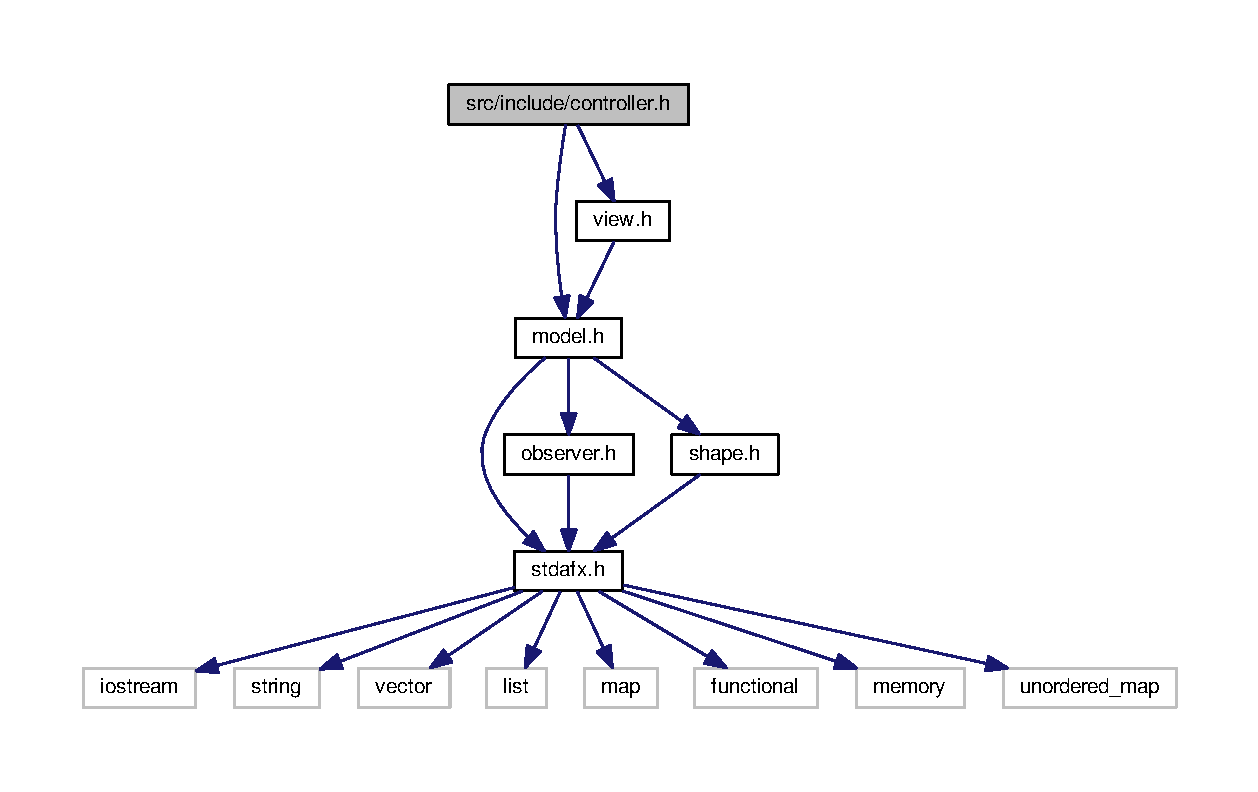
\includegraphics[width=350pt]{controller_8h__incl}
\end{center}
\end{figure}
This graph shows which files directly or indirectly include this file\-:
\nopagebreak
\begin{figure}[H]
\begin{center}
\leavevmode
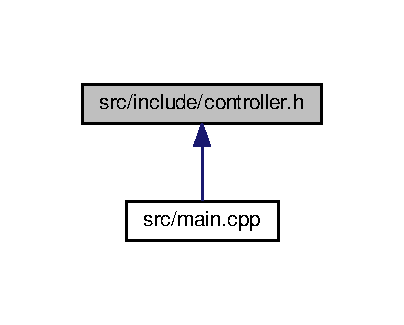
\includegraphics[width=194pt]{controller_8h__dep__incl}
\end{center}
\end{figure}

\hypertarget{model_8h}{\section{src/include/model.h File Reference}
\label{model_8h}\index{src/include/model.\-h@{src/include/model.\-h}}
}
{\ttfamily \#include $<$stdafx.\-h$>$}\\*
{\ttfamily \#include \char`\"{}observer.\-h\char`\"{}}\\*
{\ttfamily \#include \char`\"{}shape.\-h\char`\"{}}\\*
Include dependency graph for model.\-h\-:
\nopagebreak
\begin{figure}[H]
\begin{center}
\leavevmode
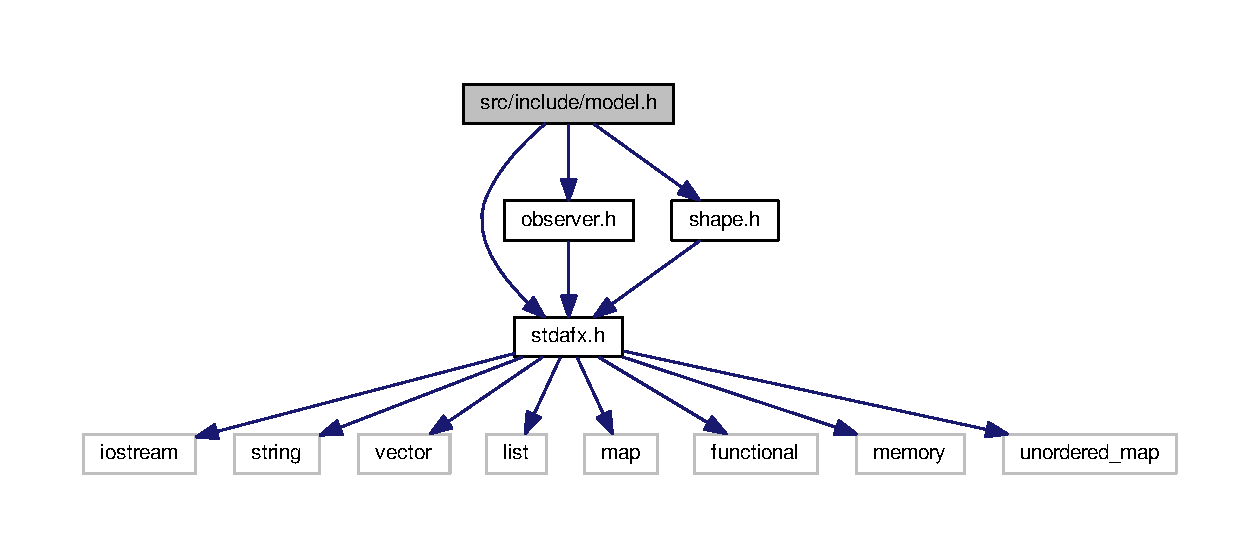
\includegraphics[width=350pt]{model_8h__incl}
\end{center}
\end{figure}
This graph shows which files directly or indirectly include this file\-:
\nopagebreak
\begin{figure}[H]
\begin{center}
\leavevmode
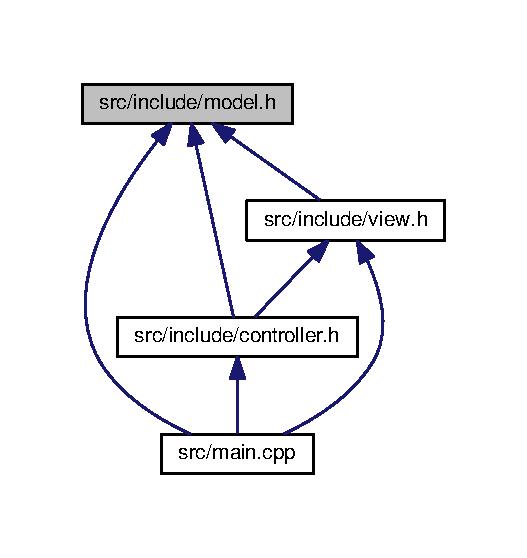
\includegraphics[width=253pt]{model_8h__dep__incl}
\end{center}
\end{figure}
\subsection*{Classes}
\begin{DoxyCompactItemize}
\item 
class \hyperlink{class_model}{Model}
\end{DoxyCompactItemize}
\subsection*{Typedefs}
\begin{DoxyCompactItemize}
\item 
using \hyperlink{model_8h_a20f87b4e5f8cd3bd25dffa8e90e1340c}{shapes\-\_\-t} = std\-::unordered\-\_\-map$<$ uint32\-\_\-t, std\-::shared\-\_\-ptr$<$ \hyperlink{class_shape}{Shape} $>$$>$
\end{DoxyCompactItemize}


\subsection{Typedef Documentation}
\hypertarget{model_8h_a20f87b4e5f8cd3bd25dffa8e90e1340c}{\index{model.\-h@{model.\-h}!shapes\-\_\-t@{shapes\-\_\-t}}
\index{shapes\-\_\-t@{shapes\-\_\-t}!model.h@{model.\-h}}
\subsubsection[{shapes\-\_\-t}]{\setlength{\rightskip}{0pt plus 5cm}using {\bf shapes\-\_\-t} =  std\-::unordered\-\_\-map$<$uint32\-\_\-t, std\-::shared\-\_\-ptr$<${\bf Shape}$>$$>$}}\label{model_8h_a20f87b4e5f8cd3bd25dffa8e90e1340c}

\hypertarget{observer_8h}{\section{src/include/observer.h File Reference}
\label{observer_8h}\index{src/include/observer.\-h@{src/include/observer.\-h}}
}
{\ttfamily \#include \char`\"{}stdafx.\-h\char`\"{}}\\*
Include dependency graph for observer.\-h\-:
\nopagebreak
\begin{figure}[H]
\begin{center}
\leavevmode
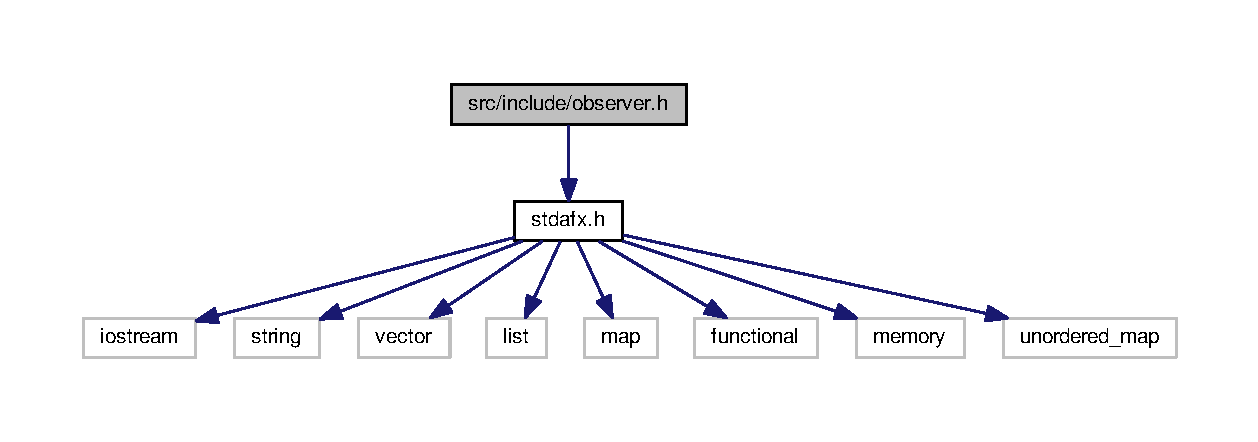
\includegraphics[width=350pt]{observer_8h__incl}
\end{center}
\end{figure}
This graph shows which files directly or indirectly include this file\-:
\nopagebreak
\begin{figure}[H]
\begin{center}
\leavevmode
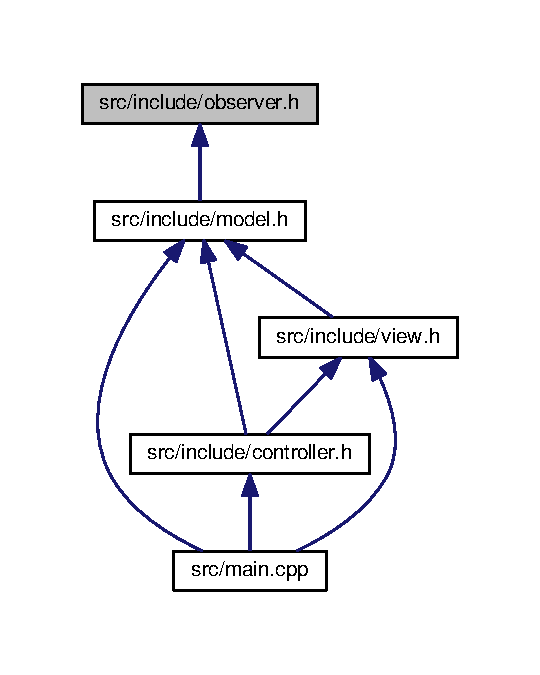
\includegraphics[width=259pt]{observer_8h__dep__incl}
\end{center}
\end{figure}
\subsection*{Classes}
\begin{DoxyCompactItemize}
\item 
class \hyperlink{class_i_observer}{I\-Observer}
\item 
class \hyperlink{class_observable}{Observable}
\end{DoxyCompactItemize}

\hypertarget{shape_8h}{\section{src/include/shape.h File Reference}
\label{shape_8h}\index{src/include/shape.\-h@{src/include/shape.\-h}}
}
{\ttfamily \#include \char`\"{}stdafx.\-h\char`\"{}}\\*
Include dependency graph for shape.\-h\-:
\nopagebreak
\begin{figure}[H]
\begin{center}
\leavevmode
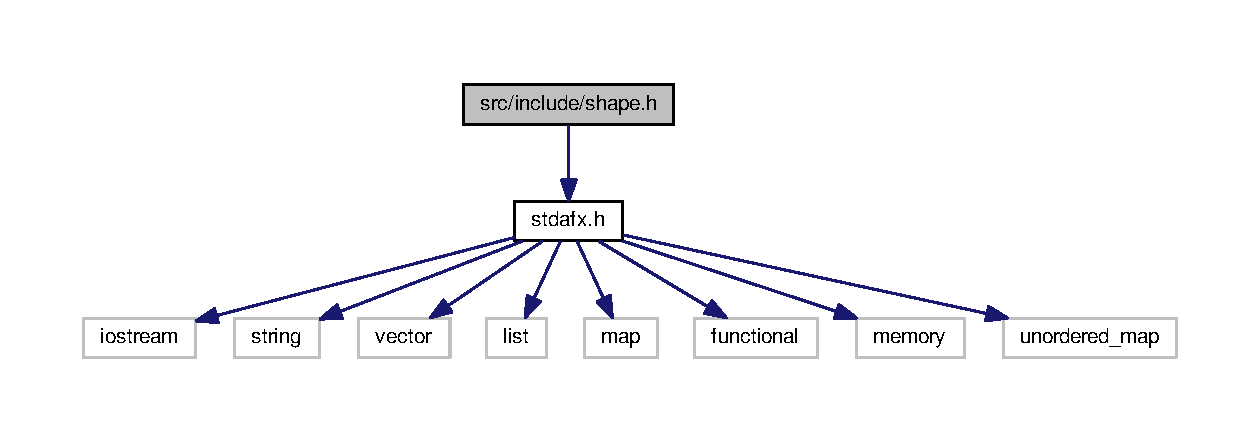
\includegraphics[width=350pt]{shape_8h__incl}
\end{center}
\end{figure}
This graph shows which files directly or indirectly include this file\-:
\nopagebreak
\begin{figure}[H]
\begin{center}
\leavevmode
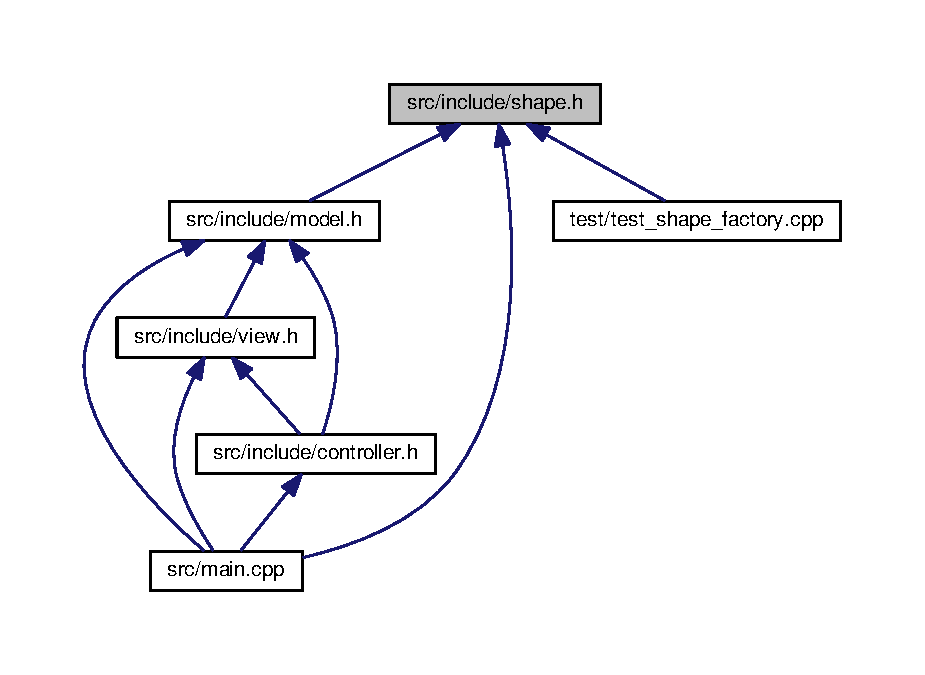
\includegraphics[width=350pt]{shape_8h__dep__incl}
\end{center}
\end{figure}
\subsection*{Classes}
\begin{DoxyCompactItemize}
\item 
class \hyperlink{class_shape}{Shape}
\item 
struct \hyperlink{struct_enum_class_hash}{Enum\-Class\-Hash}
\item 
class \hyperlink{class_shape_factory}{Shape\-Factory}
\item 
struct \hyperlink{struct_shape_factory_register}{Shape\-Factory\-Register}
\item 
class \hyperlink{class_circle}{Circle}
\item 
class \hyperlink{class_square}{Square}
\item 
class \hyperlink{class_ellipse}{Ellipse}
\end{DoxyCompactItemize}
\subsection*{Enumerations}
\begin{DoxyCompactItemize}
\item 
enum \hyperlink{shape_8h_a3c6c49dd4d974c67346f991bc443b14b}{Shapes} \{ \hyperlink{shape_8h_a3c6c49dd4d974c67346f991bc443b14baa79c827759ea48f0735386c4b1188911}{C\-I\-R\-C\-L\-E}, 
\hyperlink{shape_8h_a3c6c49dd4d974c67346f991bc443b14ba4233fbf0cafb86abcee94b38d769fc59}{S\-Q\-U\-A\-R\-E}, 
\hyperlink{shape_8h_a3c6c49dd4d974c67346f991bc443b14ba59c6b7739f239fb18fe5c81692358893}{E\-L\-L\-I\-P\-S\-E}
 \}
\end{DoxyCompactItemize}


\subsection{Enumeration Type Documentation}
\hypertarget{shape_8h_a3c6c49dd4d974c67346f991bc443b14b}{\index{shape.\-h@{shape.\-h}!Shapes@{Shapes}}
\index{Shapes@{Shapes}!shape.h@{shape.\-h}}
\subsubsection[{Shapes}]{\setlength{\rightskip}{0pt plus 5cm}enum {\bf Shapes}}}\label{shape_8h_a3c6c49dd4d974c67346f991bc443b14b}
\begin{Desc}
\item[Enumerator]\par
\begin{description}
\index{C\-I\-R\-C\-L\-E@{C\-I\-R\-C\-L\-E}!shape.\-h@{shape.\-h}}\index{shape.\-h@{shape.\-h}!C\-I\-R\-C\-L\-E@{C\-I\-R\-C\-L\-E}}\item[{\em 
\hypertarget{shape_8h_a3c6c49dd4d974c67346f991bc443b14baa79c827759ea48f0735386c4b1188911}{C\-I\-R\-C\-L\-E}\label{shape_8h_a3c6c49dd4d974c67346f991bc443b14baa79c827759ea48f0735386c4b1188911}
}]\index{S\-Q\-U\-A\-R\-E@{S\-Q\-U\-A\-R\-E}!shape.\-h@{shape.\-h}}\index{shape.\-h@{shape.\-h}!S\-Q\-U\-A\-R\-E@{S\-Q\-U\-A\-R\-E}}\item[{\em 
\hypertarget{shape_8h_a3c6c49dd4d974c67346f991bc443b14ba4233fbf0cafb86abcee94b38d769fc59}{S\-Q\-U\-A\-R\-E}\label{shape_8h_a3c6c49dd4d974c67346f991bc443b14ba4233fbf0cafb86abcee94b38d769fc59}
}]\index{E\-L\-L\-I\-P\-S\-E@{E\-L\-L\-I\-P\-S\-E}!shape.\-h@{shape.\-h}}\index{shape.\-h@{shape.\-h}!E\-L\-L\-I\-P\-S\-E@{E\-L\-L\-I\-P\-S\-E}}\item[{\em 
\hypertarget{shape_8h_a3c6c49dd4d974c67346f991bc443b14ba59c6b7739f239fb18fe5c81692358893}{E\-L\-L\-I\-P\-S\-E}\label{shape_8h_a3c6c49dd4d974c67346f991bc443b14ba59c6b7739f239fb18fe5c81692358893}
}]\end{description}
\end{Desc}

\hypertarget{stdafx_8h}{\section{src/include/stdafx.h File Reference}
\label{stdafx_8h}\index{src/include/stdafx.\-h@{src/include/stdafx.\-h}}
}
{\ttfamily \#include $<$iostream$>$}\\*
{\ttfamily \#include $<$string$>$}\\*
{\ttfamily \#include $<$vector$>$}\\*
{\ttfamily \#include $<$list$>$}\\*
{\ttfamily \#include $<$map$>$}\\*
{\ttfamily \#include $<$functional$>$}\\*
{\ttfamily \#include $<$memory$>$}\\*
{\ttfamily \#include $<$unordered\-\_\-map$>$}\\*
Include dependency graph for stdafx.\-h\-:
\nopagebreak
\begin{figure}[H]
\begin{center}
\leavevmode
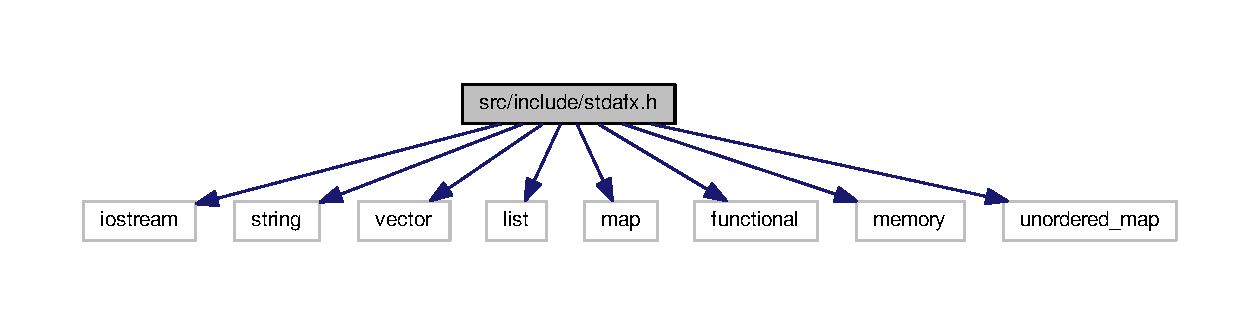
\includegraphics[width=350pt]{stdafx_8h__incl}
\end{center}
\end{figure}
This graph shows which files directly or indirectly include this file\-:
\nopagebreak
\begin{figure}[H]
\begin{center}
\leavevmode
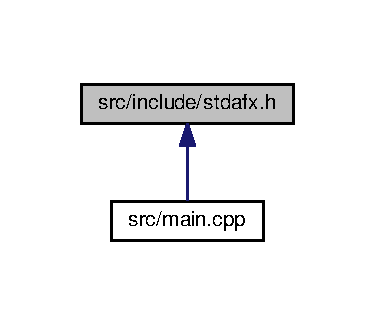
\includegraphics[width=350pt]{stdafx_8h__dep__incl}
\end{center}
\end{figure}
\subsection*{Macros}
\begin{DoxyCompactItemize}
\item 
\#define \hyperlink{stdafx_8h_a61fed2eba7bb9f87e1b1ab5f68be592a}{dout}~0 \&\& std\-::cout
\end{DoxyCompactItemize}


\subsection{Macro Definition Documentation}
\hypertarget{stdafx_8h_a61fed2eba7bb9f87e1b1ab5f68be592a}{\index{stdafx.\-h@{stdafx.\-h}!dout@{dout}}
\index{dout@{dout}!stdafx.h@{stdafx.\-h}}
\subsubsection[{dout}]{\setlength{\rightskip}{0pt plus 5cm}\#define dout~0 \&\& std\-::cout}}\label{stdafx_8h_a61fed2eba7bb9f87e1b1ab5f68be592a}

\hypertarget{view_8h}{\section{src/include/view.h File Reference}
\label{view_8h}\index{src/include/view.\-h@{src/include/view.\-h}}
}
{\ttfamily \#include \char`\"{}model.\-h\char`\"{}}\\*
Include dependency graph for view.\-h\-:
\nopagebreak
\begin{figure}[H]
\begin{center}
\leavevmode
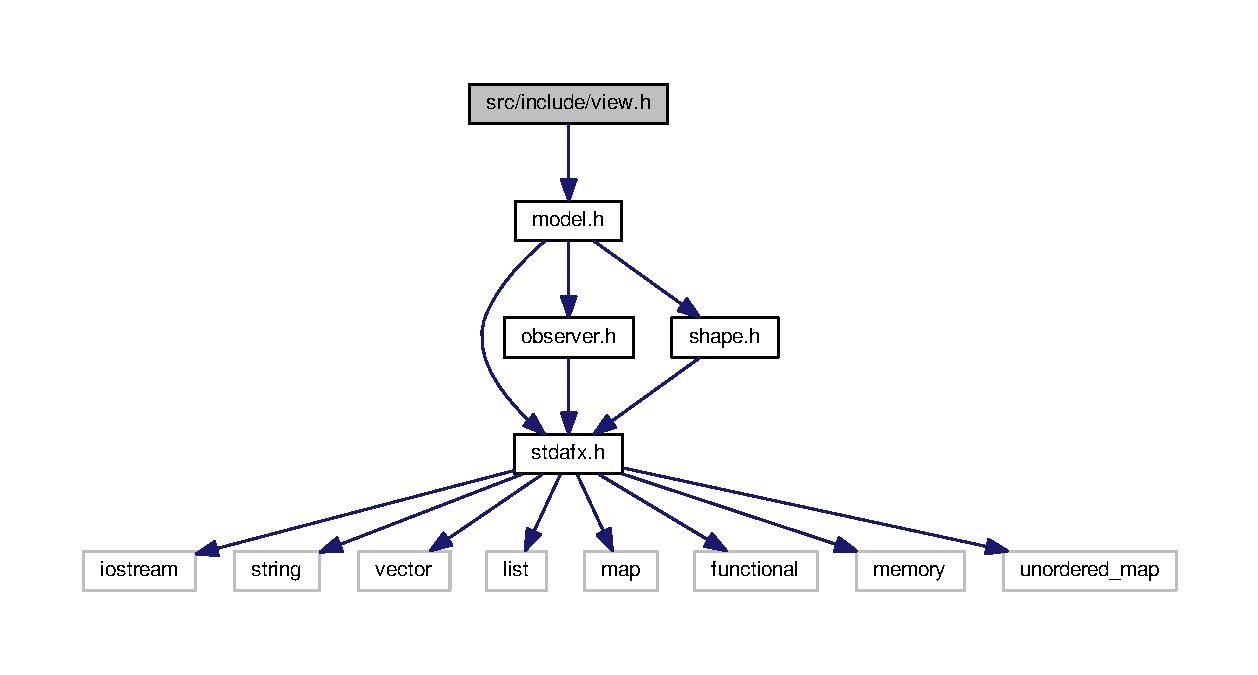
\includegraphics[width=350pt]{view_8h__incl}
\end{center}
\end{figure}
This graph shows which files directly or indirectly include this file\-:
\nopagebreak
\begin{figure}[H]
\begin{center}
\leavevmode
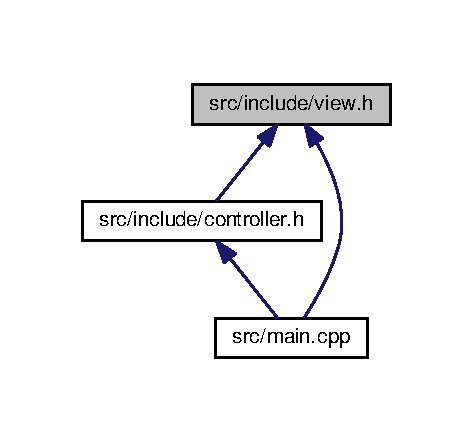
\includegraphics[width=227pt]{view_8h__dep__incl}
\end{center}
\end{figure}
\subsection*{Classes}
\begin{DoxyCompactItemize}
\item 
class \hyperlink{class_view}{View}
\end{DoxyCompactItemize}

\hypertarget{main_8cpp}{\section{src/main.cpp File Reference}
\label{main_8cpp}\index{src/main.\-cpp@{src/main.\-cpp}}
}
{\ttfamily \#include \char`\"{}stdafx.\-h\char`\"{}}\\*
Include dependency graph for main.\-cpp\-:
\nopagebreak
\begin{figure}[H]
\begin{center}
\leavevmode
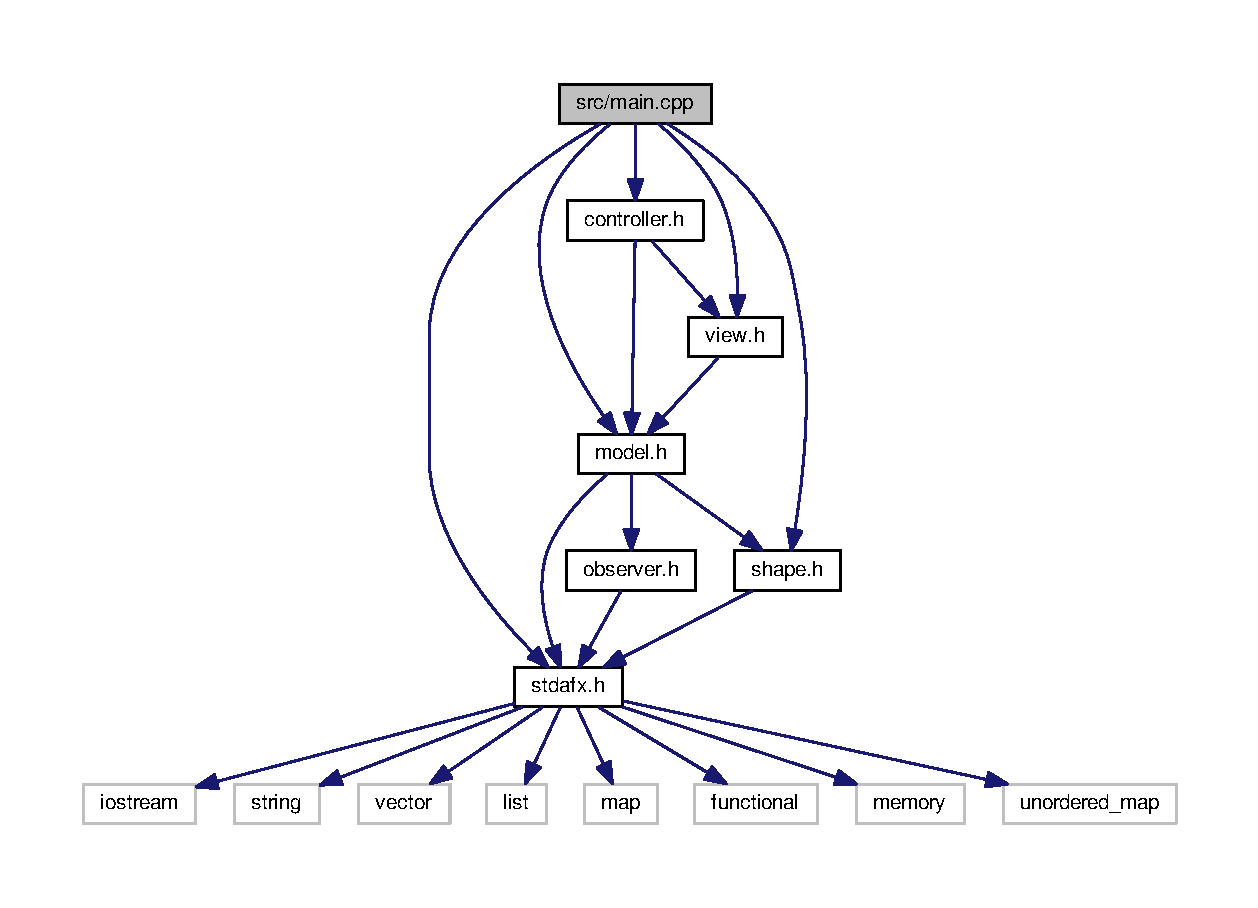
\includegraphics[width=350pt]{main_8cpp__incl}
\end{center}
\end{figure}
\subsection*{Functions}
\begin{DoxyCompactItemize}
\item 
int \hyperlink{main_8cpp_ae66f6b31b5ad750f1fe042a706a4e3d4}{main} ()
\end{DoxyCompactItemize}


\subsection{Function Documentation}
\hypertarget{main_8cpp_ae66f6b31b5ad750f1fe042a706a4e3d4}{\index{main.\-cpp@{main.\-cpp}!main@{main}}
\index{main@{main}!main.cpp@{main.\-cpp}}
\subsubsection[{main}]{\setlength{\rightskip}{0pt plus 5cm}int main (
\begin{DoxyParamCaption}
{}
\end{DoxyParamCaption}
)}}\label{main_8cpp_ae66f6b31b5ad750f1fe042a706a4e3d4}

\hypertarget{test__shape__factory_8cpp}{\section{test/test\-\_\-shape\-\_\-factory.cpp File Reference}
\label{test__shape__factory_8cpp}\index{test/test\-\_\-shape\-\_\-factory.\-cpp@{test/test\-\_\-shape\-\_\-factory.\-cpp}}
}
{\ttfamily \#include \char`\"{}stdafx.\-h\char`\"{}}\\*
{\ttfamily \#include $<$boost/test/unit\-\_\-test.\-hpp$>$}\\*
{\ttfamily \#include \char`\"{}shape.\-h\char`\"{}}\\*
{\ttfamily \#include $<$typeinfo$>$}\\*
Include dependency graph for test\-\_\-shape\-\_\-factory.\-cpp\-:
\nopagebreak
\begin{figure}[H]
\begin{center}
\leavevmode
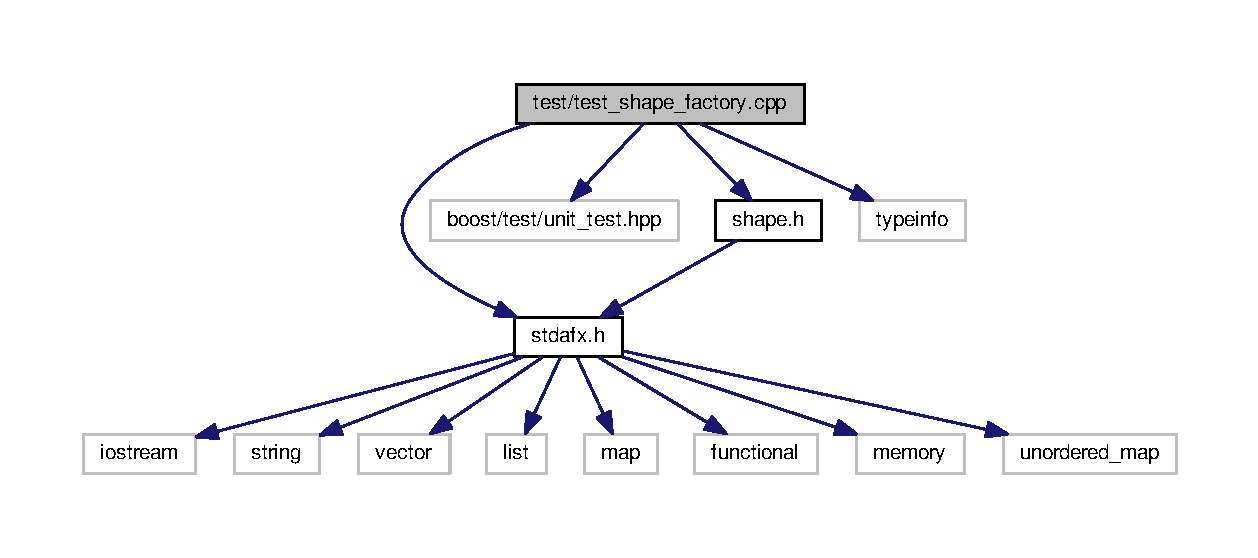
\includegraphics[width=350pt]{test__shape__factory_8cpp__incl}
\end{center}
\end{figure}
\subsection*{Macros}
\begin{DoxyCompactItemize}
\item 
\#define \hyperlink{test__shape__factory_8cpp_a6b2a3852db8bb19ab6909bac01859985}{B\-O\-O\-S\-T\-\_\-\-T\-E\-S\-T\-\_\-\-M\-O\-D\-U\-L\-E}~test\-\_\-foo
\item 
\#define \hyperlink{test__shape__factory_8cpp_a0b87e0d3bf5853bcbb0b66a7c48fdc05}{L\-O\-G\-\_\-\-L\-E\-V\-E\-L}~all
\end{DoxyCompactItemize}
\subsection*{Functions}
\begin{DoxyCompactItemize}
\item 
\hyperlink{test__shape__factory_8cpp_a91f26d41a2e866435ccae887d47893f4}{B\-O\-O\-S\-T\-\_\-\-A\-U\-T\-O\-\_\-\-T\-E\-S\-T\-\_\-\-C\-A\-S\-E} (test\-\_\-shape\-\_\-factory\-\_\-\-\_\-check\-\_\-circle\-\_\-creating)
\item 
\hyperlink{test__shape__factory_8cpp_a8c9adbb3e0113d492a7977a9cacd423d}{B\-O\-O\-S\-T\-\_\-\-A\-U\-T\-O\-\_\-\-T\-E\-S\-T\-\_\-\-C\-A\-S\-E} (test\-\_\-shape\-\_\-factory\-\_\-\-\_\-check\-\_\-ellipse\-\_\-creating)
\item 
\hyperlink{test__shape__factory_8cpp_a50c177df5e0a5f69d0dfe4c39ec4d74a}{B\-O\-O\-S\-T\-\_\-\-A\-U\-T\-O\-\_\-\-T\-E\-S\-T\-\_\-\-C\-A\-S\-E} (test\-\_\-shape\-\_\-factory\-\_\-\-\_\-check\-\_\-square\-\_\-creating)
\end{DoxyCompactItemize}


\subsection{Macro Definition Documentation}
\hypertarget{test__shape__factory_8cpp_a6b2a3852db8bb19ab6909bac01859985}{\index{test\-\_\-shape\-\_\-factory.\-cpp@{test\-\_\-shape\-\_\-factory.\-cpp}!B\-O\-O\-S\-T\-\_\-\-T\-E\-S\-T\-\_\-\-M\-O\-D\-U\-L\-E@{B\-O\-O\-S\-T\-\_\-\-T\-E\-S\-T\-\_\-\-M\-O\-D\-U\-L\-E}}
\index{B\-O\-O\-S\-T\-\_\-\-T\-E\-S\-T\-\_\-\-M\-O\-D\-U\-L\-E@{B\-O\-O\-S\-T\-\_\-\-T\-E\-S\-T\-\_\-\-M\-O\-D\-U\-L\-E}!test_shape_factory.cpp@{test\-\_\-shape\-\_\-factory.\-cpp}}
\subsubsection[{B\-O\-O\-S\-T\-\_\-\-T\-E\-S\-T\-\_\-\-M\-O\-D\-U\-L\-E}]{\setlength{\rightskip}{0pt plus 5cm}\#define B\-O\-O\-S\-T\-\_\-\-T\-E\-S\-T\-\_\-\-M\-O\-D\-U\-L\-E~test\-\_\-foo}}\label{test__shape__factory_8cpp_a6b2a3852db8bb19ab6909bac01859985}
\hypertarget{test__shape__factory_8cpp_a0b87e0d3bf5853bcbb0b66a7c48fdc05}{\index{test\-\_\-shape\-\_\-factory.\-cpp@{test\-\_\-shape\-\_\-factory.\-cpp}!L\-O\-G\-\_\-\-L\-E\-V\-E\-L@{L\-O\-G\-\_\-\-L\-E\-V\-E\-L}}
\index{L\-O\-G\-\_\-\-L\-E\-V\-E\-L@{L\-O\-G\-\_\-\-L\-E\-V\-E\-L}!test_shape_factory.cpp@{test\-\_\-shape\-\_\-factory.\-cpp}}
\subsubsection[{L\-O\-G\-\_\-\-L\-E\-V\-E\-L}]{\setlength{\rightskip}{0pt plus 5cm}\#define L\-O\-G\-\_\-\-L\-E\-V\-E\-L~all}}\label{test__shape__factory_8cpp_a0b87e0d3bf5853bcbb0b66a7c48fdc05}


\subsection{Function Documentation}
\hypertarget{test__shape__factory_8cpp_a91f26d41a2e866435ccae887d47893f4}{\index{test\-\_\-shape\-\_\-factory.\-cpp@{test\-\_\-shape\-\_\-factory.\-cpp}!B\-O\-O\-S\-T\-\_\-\-A\-U\-T\-O\-\_\-\-T\-E\-S\-T\-\_\-\-C\-A\-S\-E@{B\-O\-O\-S\-T\-\_\-\-A\-U\-T\-O\-\_\-\-T\-E\-S\-T\-\_\-\-C\-A\-S\-E}}
\index{B\-O\-O\-S\-T\-\_\-\-A\-U\-T\-O\-\_\-\-T\-E\-S\-T\-\_\-\-C\-A\-S\-E@{B\-O\-O\-S\-T\-\_\-\-A\-U\-T\-O\-\_\-\-T\-E\-S\-T\-\_\-\-C\-A\-S\-E}!test_shape_factory.cpp@{test\-\_\-shape\-\_\-factory.\-cpp}}
\subsubsection[{B\-O\-O\-S\-T\-\_\-\-A\-U\-T\-O\-\_\-\-T\-E\-S\-T\-\_\-\-C\-A\-S\-E}]{\setlength{\rightskip}{0pt plus 5cm}B\-O\-O\-S\-T\-\_\-\-A\-U\-T\-O\-\_\-\-T\-E\-S\-T\-\_\-\-C\-A\-S\-E (
\begin{DoxyParamCaption}
\item[{test\-\_\-shape\-\_\-factory\-\_\-\-\_\-check\-\_\-circle\-\_\-creating}]{}
\end{DoxyParamCaption}
)}}\label{test__shape__factory_8cpp_a91f26d41a2e866435ccae887d47893f4}
\hypertarget{test__shape__factory_8cpp_a8c9adbb3e0113d492a7977a9cacd423d}{\index{test\-\_\-shape\-\_\-factory.\-cpp@{test\-\_\-shape\-\_\-factory.\-cpp}!B\-O\-O\-S\-T\-\_\-\-A\-U\-T\-O\-\_\-\-T\-E\-S\-T\-\_\-\-C\-A\-S\-E@{B\-O\-O\-S\-T\-\_\-\-A\-U\-T\-O\-\_\-\-T\-E\-S\-T\-\_\-\-C\-A\-S\-E}}
\index{B\-O\-O\-S\-T\-\_\-\-A\-U\-T\-O\-\_\-\-T\-E\-S\-T\-\_\-\-C\-A\-S\-E@{B\-O\-O\-S\-T\-\_\-\-A\-U\-T\-O\-\_\-\-T\-E\-S\-T\-\_\-\-C\-A\-S\-E}!test_shape_factory.cpp@{test\-\_\-shape\-\_\-factory.\-cpp}}
\subsubsection[{B\-O\-O\-S\-T\-\_\-\-A\-U\-T\-O\-\_\-\-T\-E\-S\-T\-\_\-\-C\-A\-S\-E}]{\setlength{\rightskip}{0pt plus 5cm}B\-O\-O\-S\-T\-\_\-\-A\-U\-T\-O\-\_\-\-T\-E\-S\-T\-\_\-\-C\-A\-S\-E (
\begin{DoxyParamCaption}
\item[{test\-\_\-shape\-\_\-factory\-\_\-\-\_\-check\-\_\-ellipse\-\_\-creating}]{}
\end{DoxyParamCaption}
)}}\label{test__shape__factory_8cpp_a8c9adbb3e0113d492a7977a9cacd423d}
\hypertarget{test__shape__factory_8cpp_a50c177df5e0a5f69d0dfe4c39ec4d74a}{\index{test\-\_\-shape\-\_\-factory.\-cpp@{test\-\_\-shape\-\_\-factory.\-cpp}!B\-O\-O\-S\-T\-\_\-\-A\-U\-T\-O\-\_\-\-T\-E\-S\-T\-\_\-\-C\-A\-S\-E@{B\-O\-O\-S\-T\-\_\-\-A\-U\-T\-O\-\_\-\-T\-E\-S\-T\-\_\-\-C\-A\-S\-E}}
\index{B\-O\-O\-S\-T\-\_\-\-A\-U\-T\-O\-\_\-\-T\-E\-S\-T\-\_\-\-C\-A\-S\-E@{B\-O\-O\-S\-T\-\_\-\-A\-U\-T\-O\-\_\-\-T\-E\-S\-T\-\_\-\-C\-A\-S\-E}!test_shape_factory.cpp@{test\-\_\-shape\-\_\-factory.\-cpp}}
\subsubsection[{B\-O\-O\-S\-T\-\_\-\-A\-U\-T\-O\-\_\-\-T\-E\-S\-T\-\_\-\-C\-A\-S\-E}]{\setlength{\rightskip}{0pt plus 5cm}B\-O\-O\-S\-T\-\_\-\-A\-U\-T\-O\-\_\-\-T\-E\-S\-T\-\_\-\-C\-A\-S\-E (
\begin{DoxyParamCaption}
\item[{test\-\_\-shape\-\_\-factory\-\_\-\-\_\-check\-\_\-square\-\_\-creating}]{}
\end{DoxyParamCaption}
)}}\label{test__shape__factory_8cpp_a50c177df5e0a5f69d0dfe4c39ec4d74a}

%--- End generated contents ---

% Index
\newpage
\phantomsection
\addcontentsline{toc}{chapter}{Index}
\printindex

\end{document}
